%% Unit 1: An Insight to Learning
%% Included from main.tex via %% Unit 1: An Insight to Learning
%% Included from main.tex via %% Unit 1: An Insight to Learning
%% Included from main.tex via %% Unit 1: An Insight to Learning
%% Included from main.tex via \include{./units/unit1}
%% Requires the macros/colours defined in main.tex's preamble.

%==============================================================================
\section{An Insight to Learning}
%==============================================================================
\unitdivider{I}{An Insight to Learning}{Learning, memory, emotion \& empathy}

\begin{frame}{Understanding the Learning Process}
  \accentrule\\[0.3em]
  \begin{columns}[T]
    \begin{column}{0.58\textwidth}\small
      Learning is the process of acquiring \kw{knowledge}, \kw{skills} and
      \kw{attitudes} through experience, study or teaching.
      \begin{itemize}\small
        \item \kwt{Cognitive} — thinking, understanding, problem solving.
        \item \kwt{Affective} — emotions, values, motivation.
        \item \kwt{Psychomotor} — physical / hands-on skills.
      \end{itemize}
      \vspace{0.3em}
      Effective designers are \emph{lifelong learners}: they observe, reflect,
      conceptualise and experiment — exactly the loop Kolb described.
    \end{column}
    \begin{column}{0.42\textwidth}
      \begin{block}{Why it matters for design}
        \scriptsize
        Understanding \emph{how humans learn} helps us design products,
        instructions and experiences that people can pick up quickly and use
        intuitively.
      \end{block}
    \end{column}
  \end{columns}
\end{frame}

\begin{frame}{Kolb's Experiential Learning Cycle}
  \begin{columns}[c]
    \begin{column}{0.55\textwidth}
      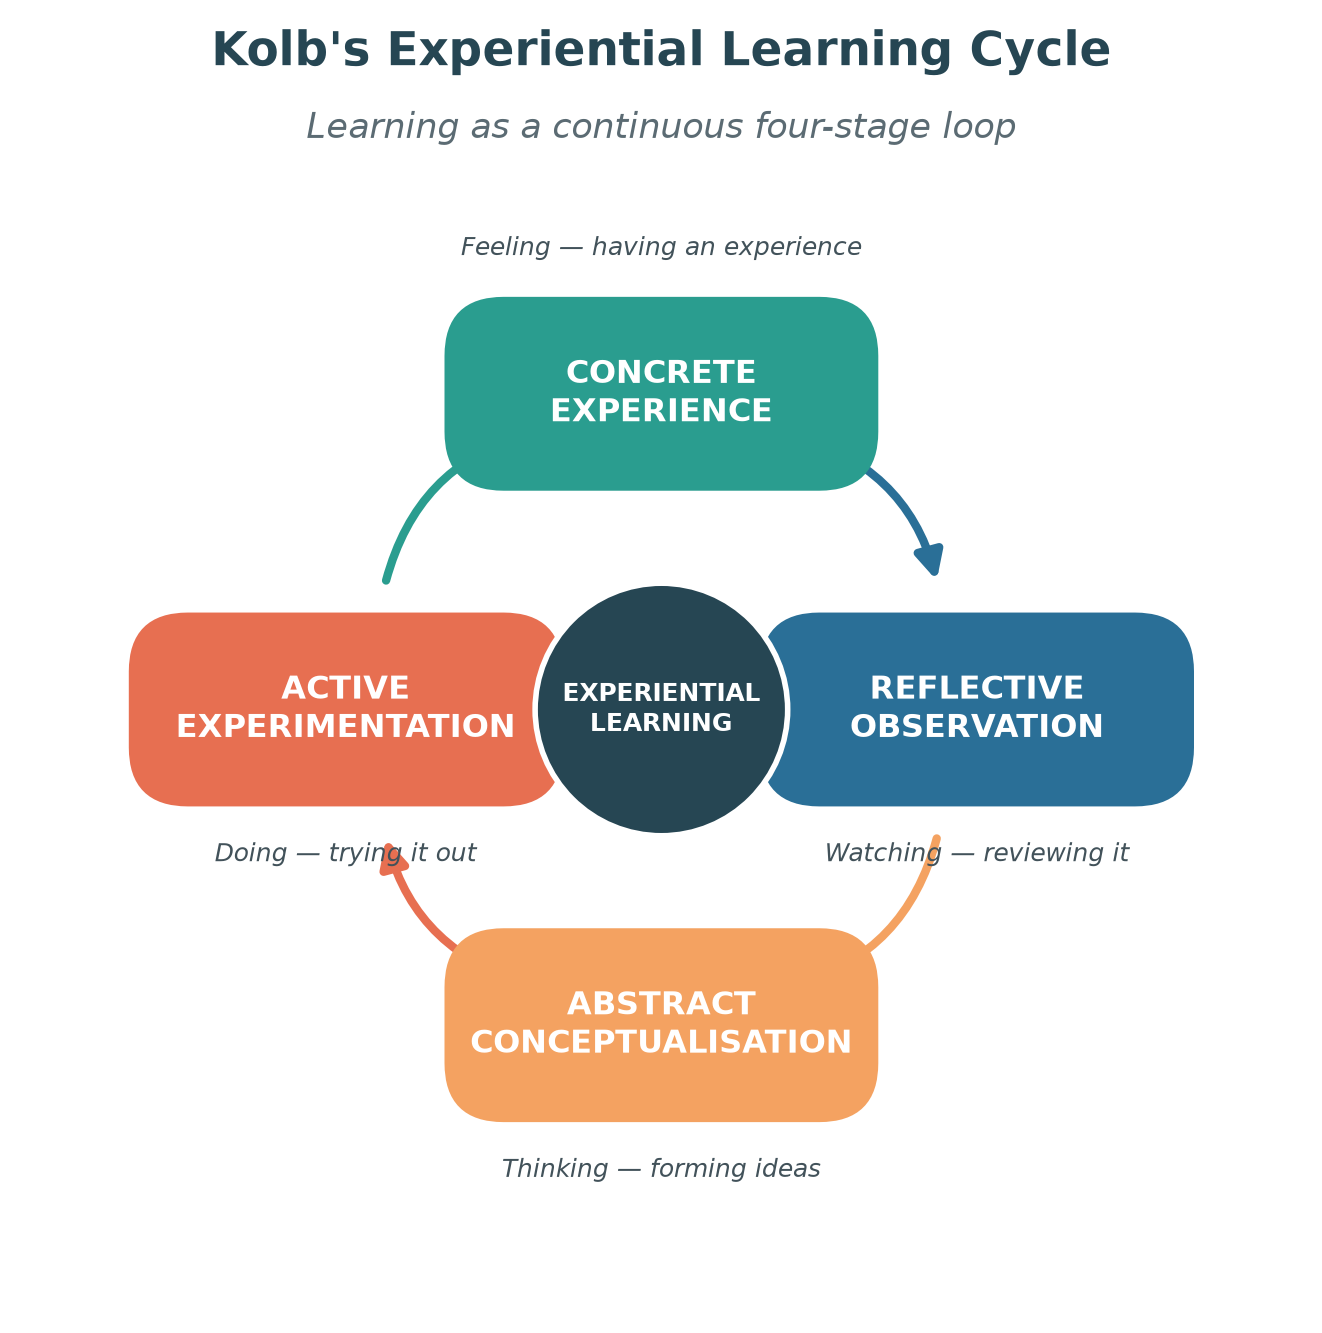
\includegraphics[width=\linewidth]{figures/kolb_cycle.png}
    \end{column}
    \begin{column}{0.45\textwidth}\footnotesize
      Learning is a \kw{continuous cycle} of four stages:
      \begin{enumerate}\footnotesize
        \item \kwt{Concrete Experience} — do / feel.
        \item \kwt{Reflective Observation} — review.
        \item \kwt{Abstract Conceptualisation} — conclude.
        \item \kwt{Active Experimentation} — plan \& try.
      \end{enumerate}
      Effective learning happens when we travel \emph{all the way round} the
      loop — repeatedly.
    \end{column}
  \end{columns}
\end{frame}

\begin{frame}{Kolb's Four Learning Styles}
  \begin{columns}[c]
    \begin{column}{0.58\textwidth}
      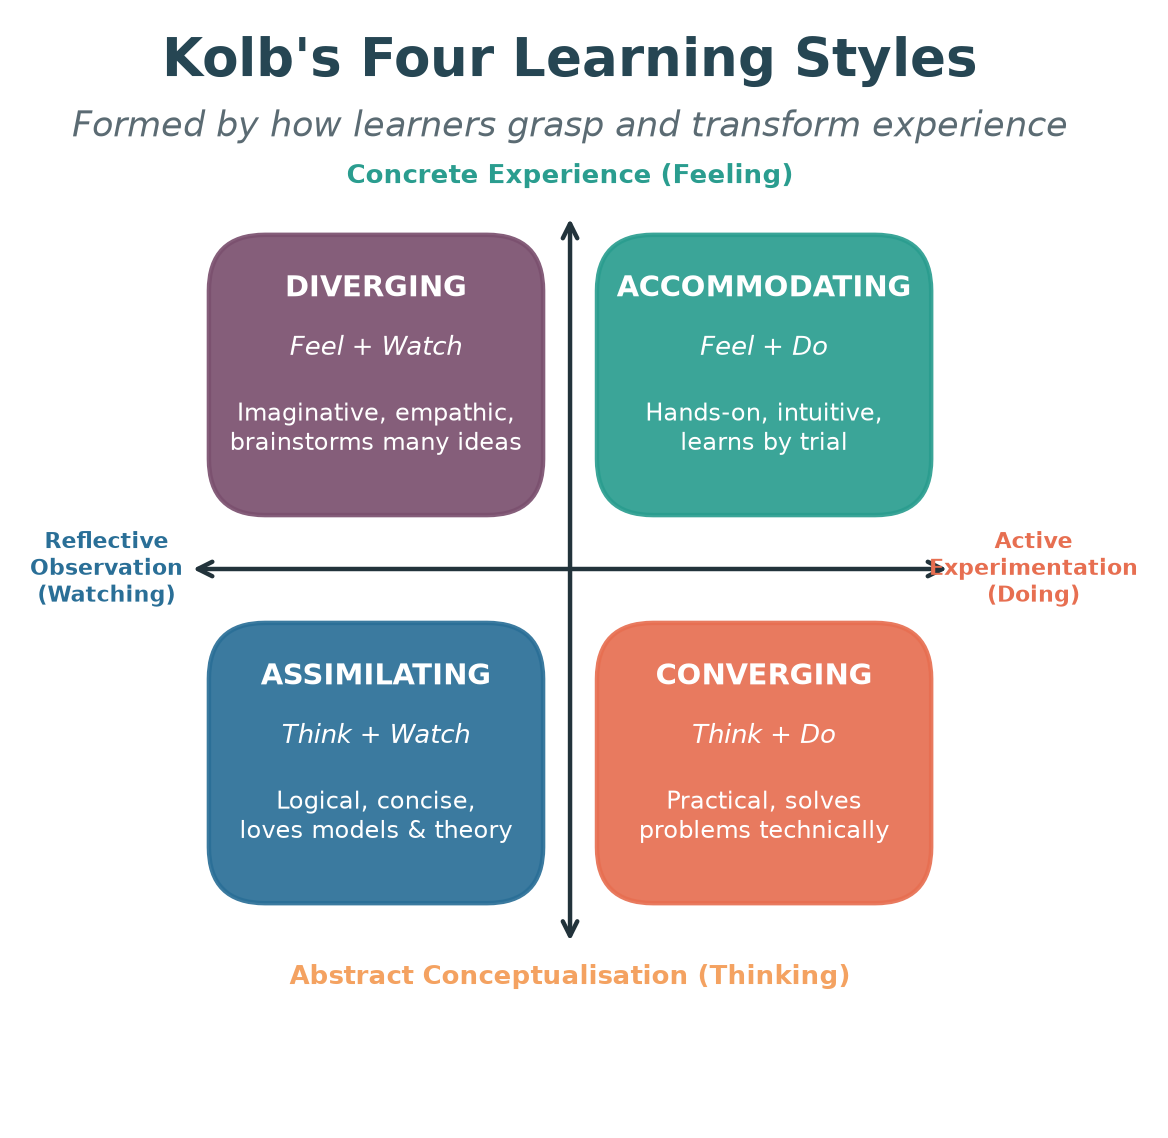
\includegraphics[width=\linewidth]{figures/kolb_styles.png}
    \end{column}
    \begin{column}{0.42\textwidth}\scriptsize
      Combining \emph{how we grasp} and \emph{how we transform} experience
      gives four styles:
      \begin{itemize}\scriptsize
        \item \pill{dtplum}{Diverging} — imaginative, many ideas.
        \item \pill{dtteal}{Accommodating} — hands-on, intuitive.
        \item \pill{dtblue}{Assimilating} — logical, loves theory.
        \item \pill{dtcoral}{Converging} — practical problem-solver.
      \end{itemize}
      \vspace{0.3em}
      Teams work best when \emph{all four styles} are present.
    \end{column}
  \end{columns}
\end{frame}

\begin{frame}{Assessing \& Interpreting Learning Styles}
  \accentrule\\[0.3em]
  \begin{columns}[T]
    \begin{column}{0.5\textwidth}\small
      \textbf{How we assess}
      \begin{itemize}\small
        \item \kw{Learning Style Inventory (LSI)} questionnaires.
        \item Self-reflection journals.
        \item Observation of behaviour in tasks.
      \end{itemize}
    \end{column}
    \begin{column}{0.5\textwidth}\small
      \textbf{How we interpret}
      \begin{itemize}\small
        \item No style is \emph{better} — each has strengths.
        \item Match \kwt{teaching methods} to styles.
        \item Encourage learners to stretch into weaker modes.
      \end{itemize}
    \end{column}
  \end{columns}
  \vspace{0.4em}
  \begin{block}{Application with peers}
    \scriptsize In group projects, deliberately mix styles so ideation,
    analysis, building and testing are all covered.
  \end{block}
\end{frame}

\begin{frame}{The Memory Process}
  \bigfig{memory_process.png}{The information-processing model: sensory $\to$ short-term $\to$ long-term memory.}
\end{frame}

\begin{frame}{Problems in Retention}
  \accentrule\\[0.3em]
  \begin{columns}[T]
    \begin{column}{0.5\textwidth}\small
      Why do we forget?
      \begin{itemize}\small
        \item \kwc{Decay} — traces fade without use.
        \item \kwc{Interference} — old \& new memories clash.
        \item \kwc{Retrieval failure} — no cue to recall.
        \item \kwc{Weak encoding} — shallow processing.
      \end{itemize}
    \end{column}
    \begin{column}{0.5\textwidth}
      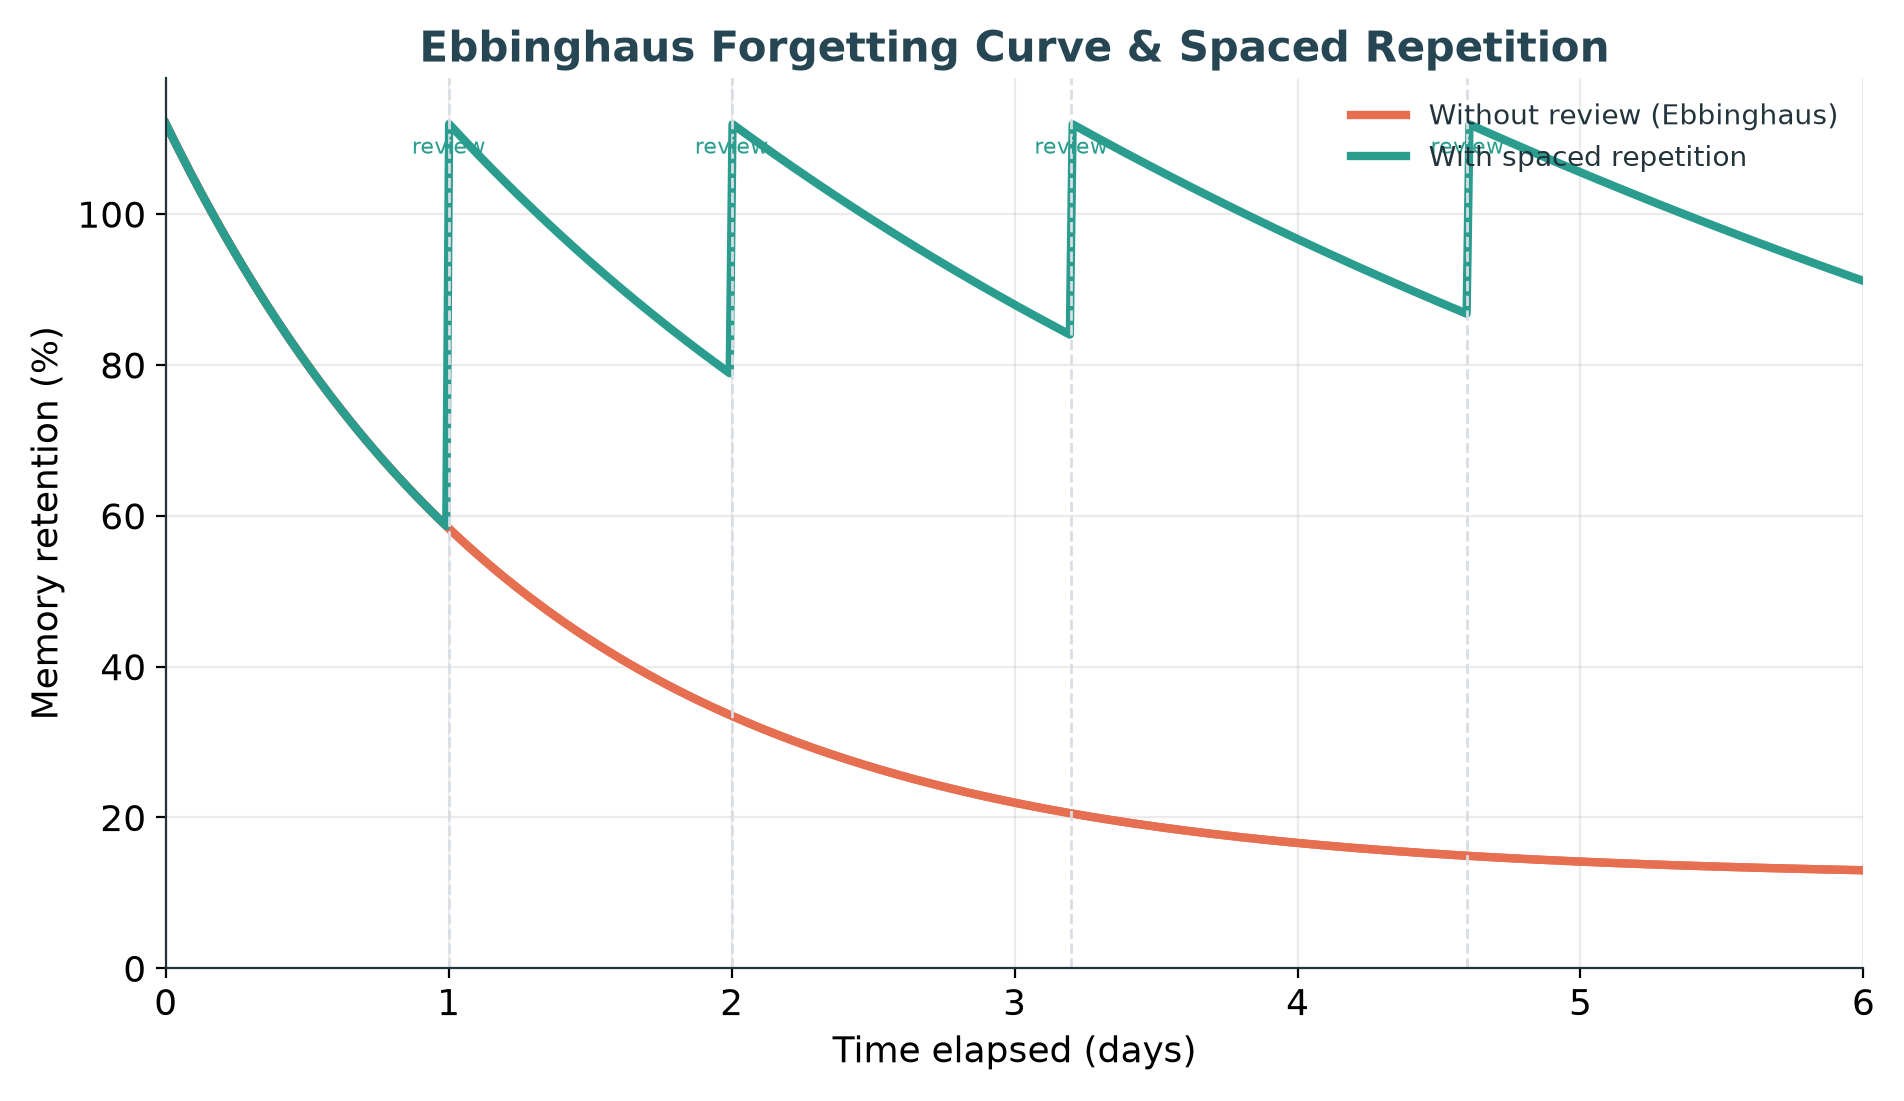
\includegraphics[width=\linewidth]{figures/forgetting_curve.png}
    \end{column}
  \end{columns}
  \vspace{0.2em}
  {\scriptsize The \kw{Ebbinghaus curve} shows rapid forgetting — but each
  review flattens the curve.}
\end{frame}

\begin{frame}{Memory Enhancement Techniques}
  \accentrule\\[0.4em]
  \begin{columns}[T]
    \begin{column}{0.5\textwidth}\small
      \begin{itemize}\small
        \item \kwt{Chunking} — group items into meaningful units.
        \item \kwt{Mnemonics} — acronyms, rhymes, imagery.
        \item \kwt{Spaced repetition} — review at intervals.
        \item \kwt{Elaboration} — connect to prior knowledge.
      \end{itemize}
    \end{column}
    \begin{column}{0.5\textwidth}\small
      \begin{itemize}\small
        \item \kwt{Dual coding} — words + visuals together.
        \item \kwt{Active recall} — test yourself, don't re-read.
        \item \kwt{Method of loci} — memory "palace".
        \item \kwt{Sleep \& rest} — consolidate memories.
      \end{itemize}
    \end{column}
  \end{columns}
  \vspace{0.4em}
  \begin{block}{Design tip}\scriptsize
    Good product design \emph{reduces the memory load} on the user — clear
    labels, consistent layouts and helpful cues.
  \end{block}
\end{frame}

\begin{frame}{Emotions, Experience \& Expression}
  \accentrule\\[0.3em]
  \begin{columns}[T]
    \begin{column}{0.55\textwidth}\small
      Emotions shape how people \kw{experience} and \kw{remember} products.
      \begin{itemize}\small
        \item \kwt{Emotion} — an internal feeling (joy, frustration, trust).
        \item \kwt{Experience} — the felt journey of using something.
        \item \kwt{Expression} — how emotion is shown \& communicated.
      \end{itemize}
      \vspace{0.3em}
      Peak emotions (delight or annoyance) leave the strongest memories —
      the \emph{peak-end rule}.
    \end{column}
    \begin{column}{0.45\textwidth}
      \begin{block}{Emotional design (Norman)}\scriptsize
        \begin{itemize}\scriptsize
          \item \textbf{Visceral} — first look \& feel.
          \item \textbf{Behavioural} — pleasure of use.
          \item \textbf{Reflective} — meaning \& self-image.
        \end{itemize}
      \end{block}
    \end{column}
  \end{columns}
\end{frame}

\begin{frame}{Empathy \& Emotional Intelligence}
  \begin{columns}[c]
    \begin{column}{0.6\textwidth}
      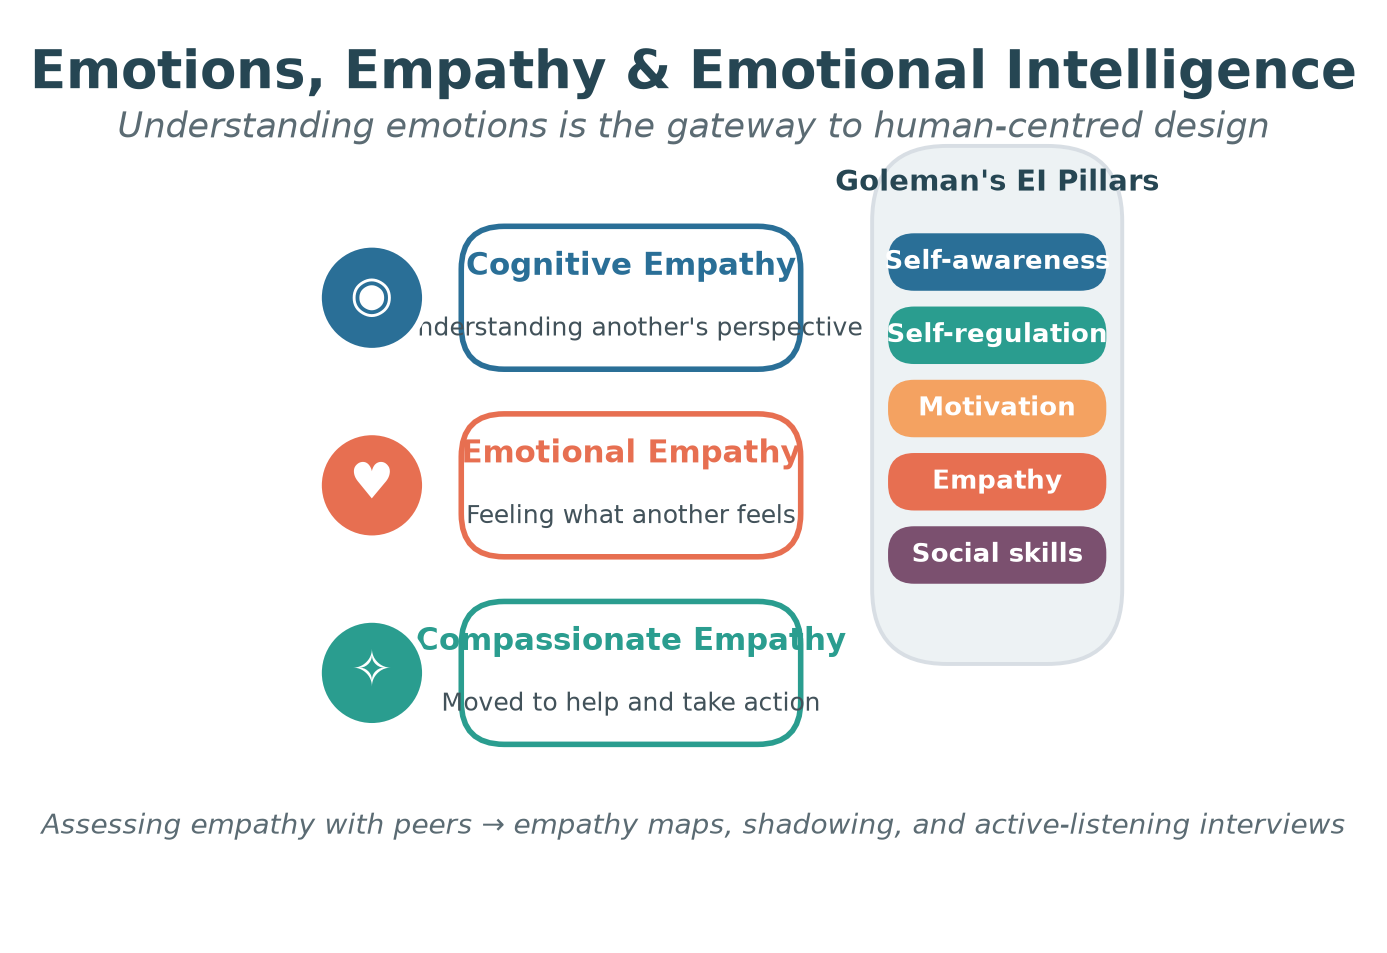
\includegraphics[width=\linewidth]{figures/empathy.png}
    \end{column}
    \begin{column}{0.4\textwidth}\scriptsize
      \kw{Empathy} — the ability to understand and share another's feelings —
      is the \emph{heart of design thinking}.
      \vspace{0.3em}
      \textbf{Assessing empathy with peers}
      \begin{itemize}\scriptsize
        \item Empathy maps (says / thinks / does / feels).
        \item Shadowing \& observation.
        \item Active-listening interviews.
      \end{itemize}
    \end{column}
  \end{columns}
\end{frame}

%% Requires the macros/colours defined in main.tex's preamble.

%==============================================================================
\section{An Insight to Learning}
%==============================================================================
\unitdivider{I}{An Insight to Learning}{Learning, memory, emotion \& empathy}

\begin{frame}{Understanding the Learning Process}
  \accentrule\\[0.3em]
  \begin{columns}[T]
    \begin{column}{0.58\textwidth}\small
      Learning is the process of acquiring \kw{knowledge}, \kw{skills} and
      \kw{attitudes} through experience, study or teaching.
      \begin{itemize}\small
        \item \kwt{Cognitive} — thinking, understanding, problem solving.
        \item \kwt{Affective} — emotions, values, motivation.
        \item \kwt{Psychomotor} — physical / hands-on skills.
      \end{itemize}
      \vspace{0.3em}
      Effective designers are \emph{lifelong learners}: they observe, reflect,
      conceptualise and experiment — exactly the loop Kolb described.
    \end{column}
    \begin{column}{0.42\textwidth}
      \begin{block}{Why it matters for design}
        \scriptsize
        Understanding \emph{how humans learn} helps us design products,
        instructions and experiences that people can pick up quickly and use
        intuitively.
      \end{block}
    \end{column}
  \end{columns}
\end{frame}

\begin{frame}{Kolb's Experiential Learning Cycle}
  \begin{columns}[c]
    \begin{column}{0.55\textwidth}
      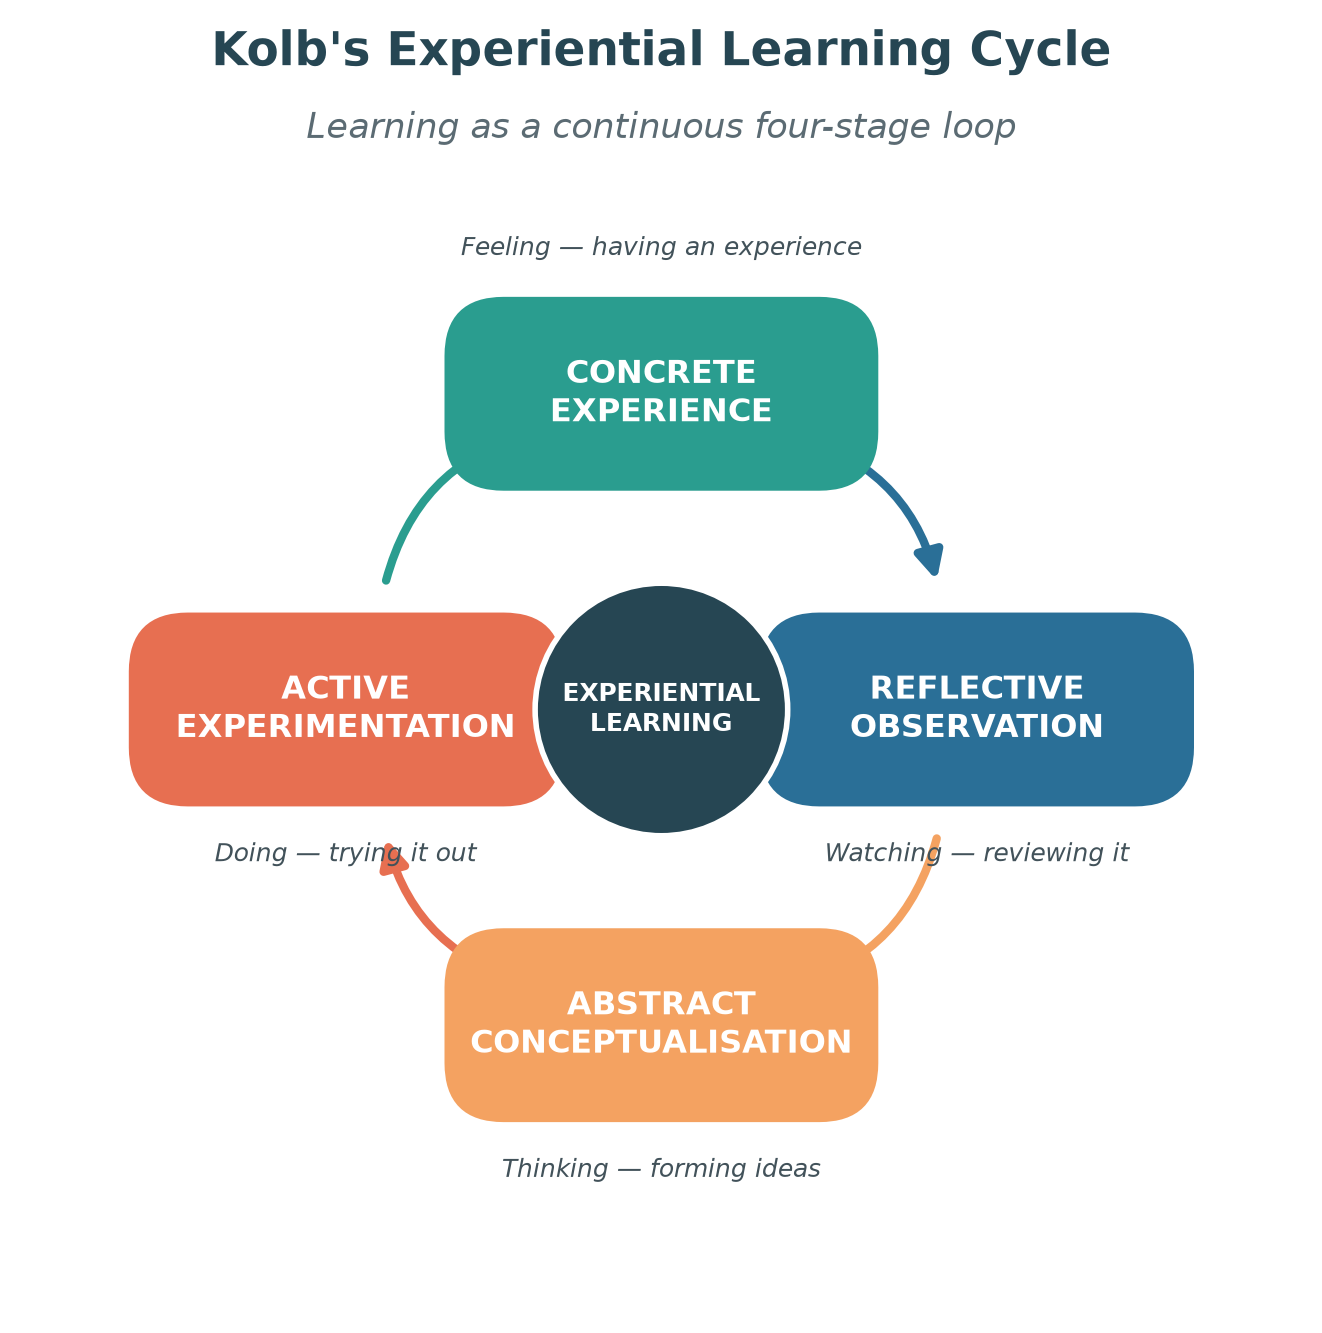
\includegraphics[width=\linewidth]{figures/kolb_cycle.png}
    \end{column}
    \begin{column}{0.45\textwidth}\footnotesize
      Learning is a \kw{continuous cycle} of four stages:
      \begin{enumerate}\footnotesize
        \item \kwt{Concrete Experience} — do / feel.
        \item \kwt{Reflective Observation} — review.
        \item \kwt{Abstract Conceptualisation} — conclude.
        \item \kwt{Active Experimentation} — plan \& try.
      \end{enumerate}
      Effective learning happens when we travel \emph{all the way round} the
      loop — repeatedly.
    \end{column}
  \end{columns}
\end{frame}

\begin{frame}{Kolb's Four Learning Styles}
  \begin{columns}[c]
    \begin{column}{0.58\textwidth}
      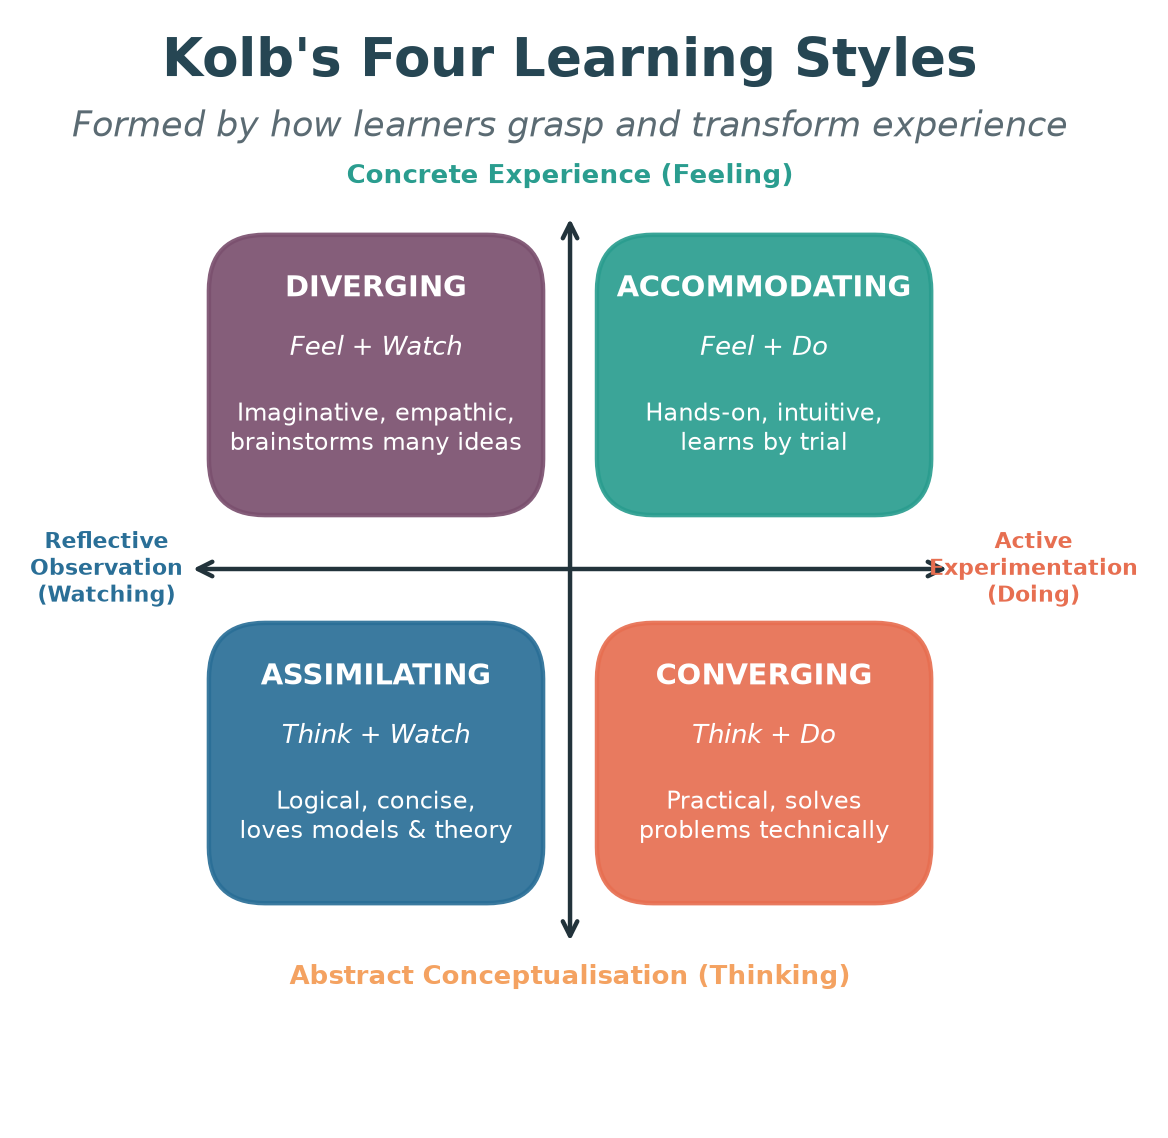
\includegraphics[width=\linewidth]{figures/kolb_styles.png}
    \end{column}
    \begin{column}{0.42\textwidth}\scriptsize
      Combining \emph{how we grasp} and \emph{how we transform} experience
      gives four styles:
      \begin{itemize}\scriptsize
        \item \pill{dtplum}{Diverging} — imaginative, many ideas.
        \item \pill{dtteal}{Accommodating} — hands-on, intuitive.
        \item \pill{dtblue}{Assimilating} — logical, loves theory.
        \item \pill{dtcoral}{Converging} — practical problem-solver.
      \end{itemize}
      \vspace{0.3em}
      Teams work best when \emph{all four styles} are present.
    \end{column}
  \end{columns}
\end{frame}

\begin{frame}{Assessing \& Interpreting Learning Styles}
  \accentrule\\[0.3em]
  \begin{columns}[T]
    \begin{column}{0.5\textwidth}\small
      \textbf{How we assess}
      \begin{itemize}\small
        \item \kw{Learning Style Inventory (LSI)} questionnaires.
        \item Self-reflection journals.
        \item Observation of behaviour in tasks.
      \end{itemize}
    \end{column}
    \begin{column}{0.5\textwidth}\small
      \textbf{How we interpret}
      \begin{itemize}\small
        \item No style is \emph{better} — each has strengths.
        \item Match \kwt{teaching methods} to styles.
        \item Encourage learners to stretch into weaker modes.
      \end{itemize}
    \end{column}
  \end{columns}
  \vspace{0.4em}
  \begin{block}{Application with peers}
    \scriptsize In group projects, deliberately mix styles so ideation,
    analysis, building and testing are all covered.
  \end{block}
\end{frame}

\begin{frame}{The Memory Process}
  \bigfig{memory_process.png}{The information-processing model: sensory $\to$ short-term $\to$ long-term memory.}
\end{frame}

\begin{frame}{Problems in Retention}
  \accentrule\\[0.3em]
  \begin{columns}[T]
    \begin{column}{0.5\textwidth}\small
      Why do we forget?
      \begin{itemize}\small
        \item \kwc{Decay} — traces fade without use.
        \item \kwc{Interference} — old \& new memories clash.
        \item \kwc{Retrieval failure} — no cue to recall.
        \item \kwc{Weak encoding} — shallow processing.
      \end{itemize}
    \end{column}
    \begin{column}{0.5\textwidth}
      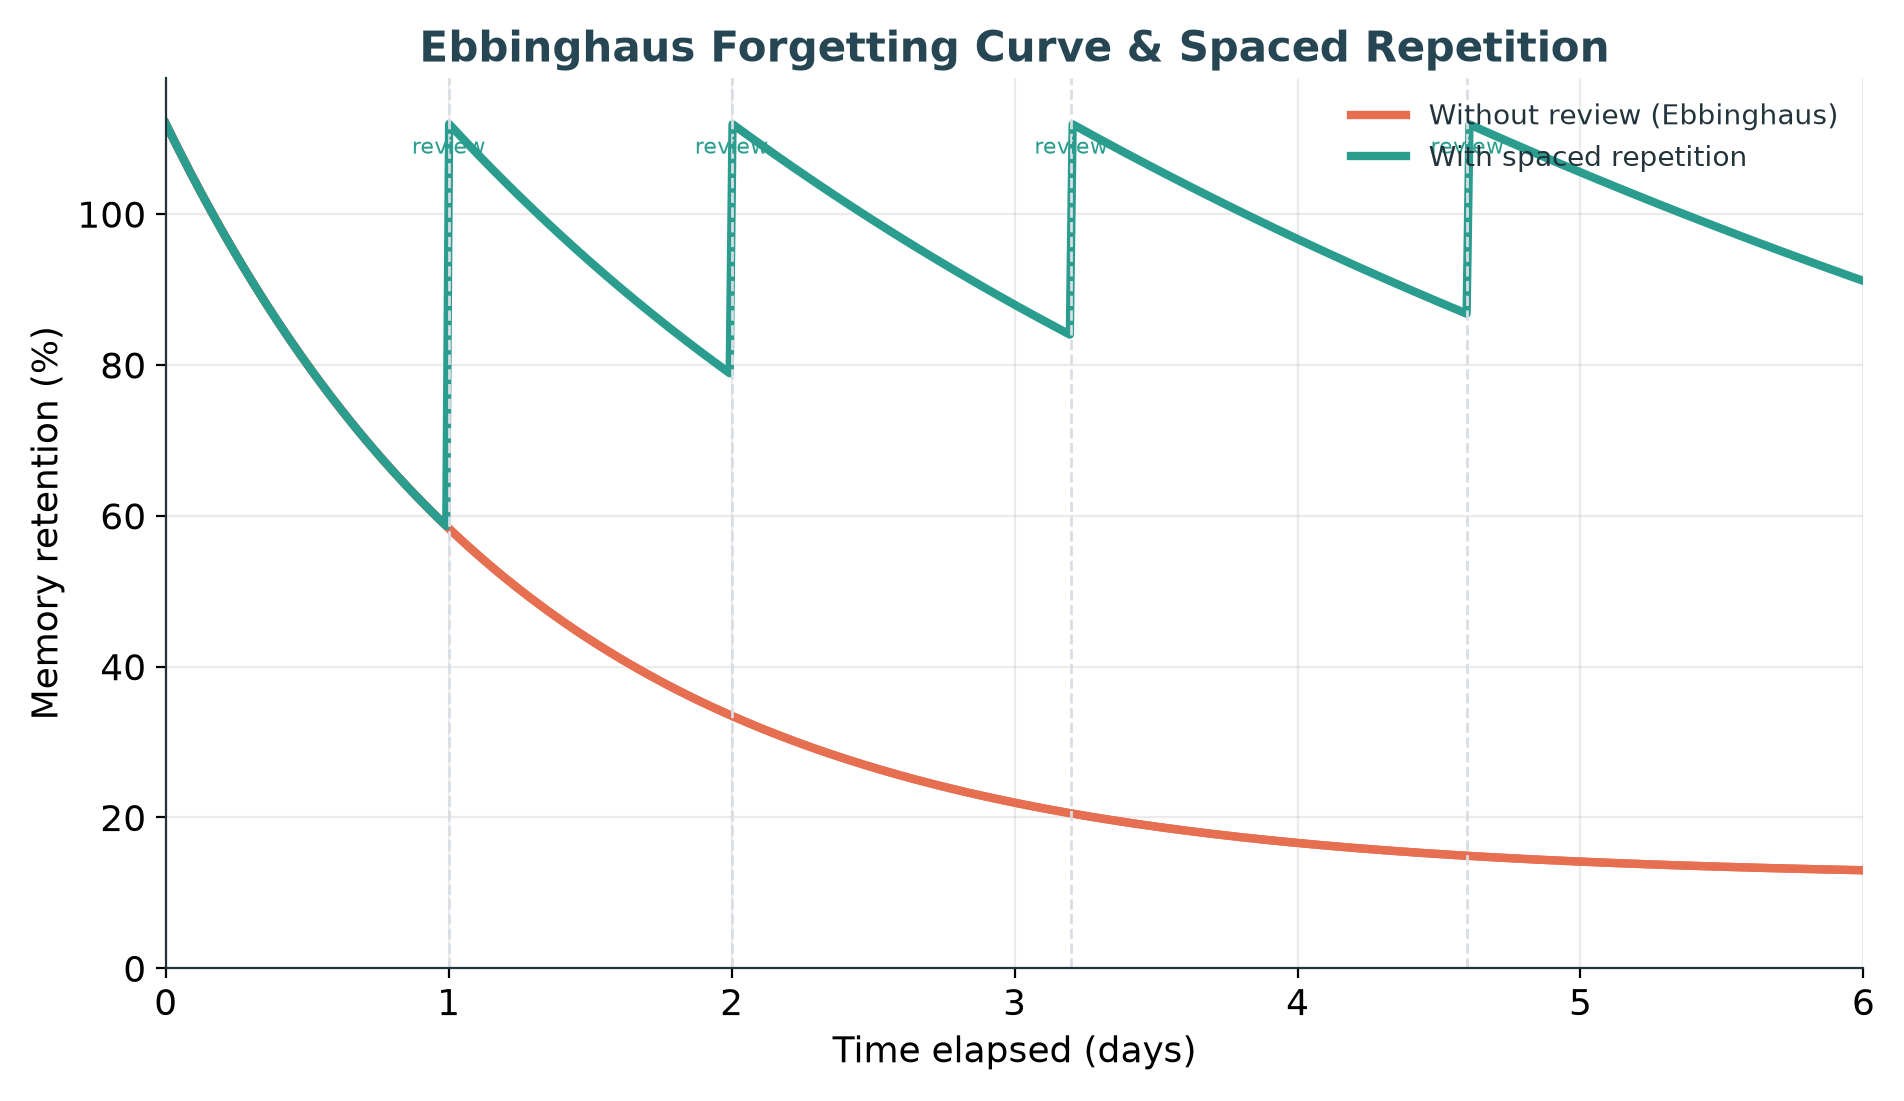
\includegraphics[width=\linewidth]{figures/forgetting_curve.png}
    \end{column}
  \end{columns}
  \vspace{0.2em}
  {\scriptsize The \kw{Ebbinghaus curve} shows rapid forgetting — but each
  review flattens the curve.}
\end{frame}

\begin{frame}{Memory Enhancement Techniques}
  \accentrule\\[0.4em]
  \begin{columns}[T]
    \begin{column}{0.5\textwidth}\small
      \begin{itemize}\small
        \item \kwt{Chunking} — group items into meaningful units.
        \item \kwt{Mnemonics} — acronyms, rhymes, imagery.
        \item \kwt{Spaced repetition} — review at intervals.
        \item \kwt{Elaboration} — connect to prior knowledge.
      \end{itemize}
    \end{column}
    \begin{column}{0.5\textwidth}\small
      \begin{itemize}\small
        \item \kwt{Dual coding} — words + visuals together.
        \item \kwt{Active recall} — test yourself, don't re-read.
        \item \kwt{Method of loci} — memory "palace".
        \item \kwt{Sleep \& rest} — consolidate memories.
      \end{itemize}
    \end{column}
  \end{columns}
  \vspace{0.4em}
  \begin{block}{Design tip}\scriptsize
    Good product design \emph{reduces the memory load} on the user — clear
    labels, consistent layouts and helpful cues.
  \end{block}
\end{frame}

\begin{frame}{Emotions, Experience \& Expression}
  \accentrule\\[0.3em]
  \begin{columns}[T]
    \begin{column}{0.55\textwidth}\small
      Emotions shape how people \kw{experience} and \kw{remember} products.
      \begin{itemize}\small
        \item \kwt{Emotion} — an internal feeling (joy, frustration, trust).
        \item \kwt{Experience} — the felt journey of using something.
        \item \kwt{Expression} — how emotion is shown \& communicated.
      \end{itemize}
      \vspace{0.3em}
      Peak emotions (delight or annoyance) leave the strongest memories —
      the \emph{peak-end rule}.
    \end{column}
    \begin{column}{0.45\textwidth}
      \begin{block}{Emotional design (Norman)}\scriptsize
        \begin{itemize}\scriptsize
          \item \textbf{Visceral} — first look \& feel.
          \item \textbf{Behavioural} — pleasure of use.
          \item \textbf{Reflective} — meaning \& self-image.
        \end{itemize}
      \end{block}
    \end{column}
  \end{columns}
\end{frame}

\begin{frame}{Empathy \& Emotional Intelligence}
  \begin{columns}[c]
    \begin{column}{0.6\textwidth}
      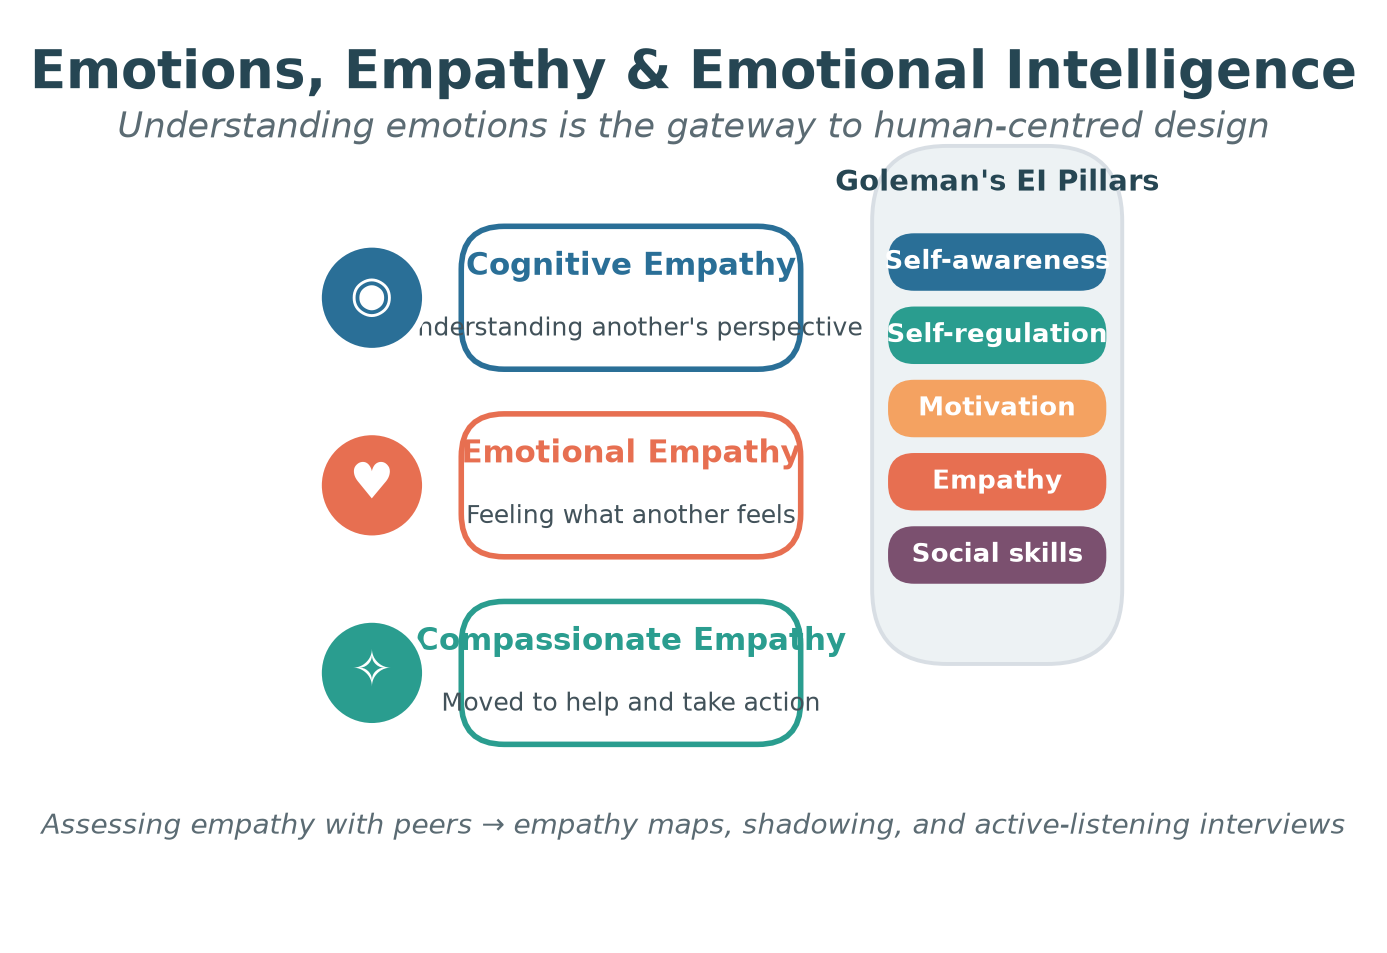
\includegraphics[width=\linewidth]{figures/empathy.png}
    \end{column}
    \begin{column}{0.4\textwidth}\scriptsize
      \kw{Empathy} — the ability to understand and share another's feelings —
      is the \emph{heart of design thinking}.
      \vspace{0.3em}
      \textbf{Assessing empathy with peers}
      \begin{itemize}\scriptsize
        \item Empathy maps (says / thinks / does / feels).
        \item Shadowing \& observation.
        \item Active-listening interviews.
      \end{itemize}
    \end{column}
  \end{columns}
\end{frame}

%% Requires the macros/colours defined in main.tex's preamble.

%==============================================================================
\section{An Insight to Learning}
%==============================================================================
\unitdivider{I}{An Insight to Learning}{Learning, memory, emotion \& empathy}

\begin{frame}{Understanding the Learning Process}
  \accentrule\\[0.3em]
  \begin{columns}[T]
    \begin{column}{0.58\textwidth}\small
      Learning is the process of acquiring \kw{knowledge}, \kw{skills} and
      \kw{attitudes} through experience, study or teaching.
      \begin{itemize}\small
        \item \kwt{Cognitive} — thinking, understanding, problem solving.
        \item \kwt{Affective} — emotions, values, motivation.
        \item \kwt{Psychomotor} — physical / hands-on skills.
      \end{itemize}
      \vspace{0.3em}
      Effective designers are \emph{lifelong learners}: they observe, reflect,
      conceptualise and experiment — exactly the loop Kolb described.
    \end{column}
    \begin{column}{0.42\textwidth}
      \begin{block}{Why it matters for design}
        \scriptsize
        Understanding \emph{how humans learn} helps us design products,
        instructions and experiences that people can pick up quickly and use
        intuitively.
      \end{block}
    \end{column}
  \end{columns}
\end{frame}

\begin{frame}{Kolb's Experiential Learning Cycle}
  \begin{columns}[c]
    \begin{column}{0.55\textwidth}
      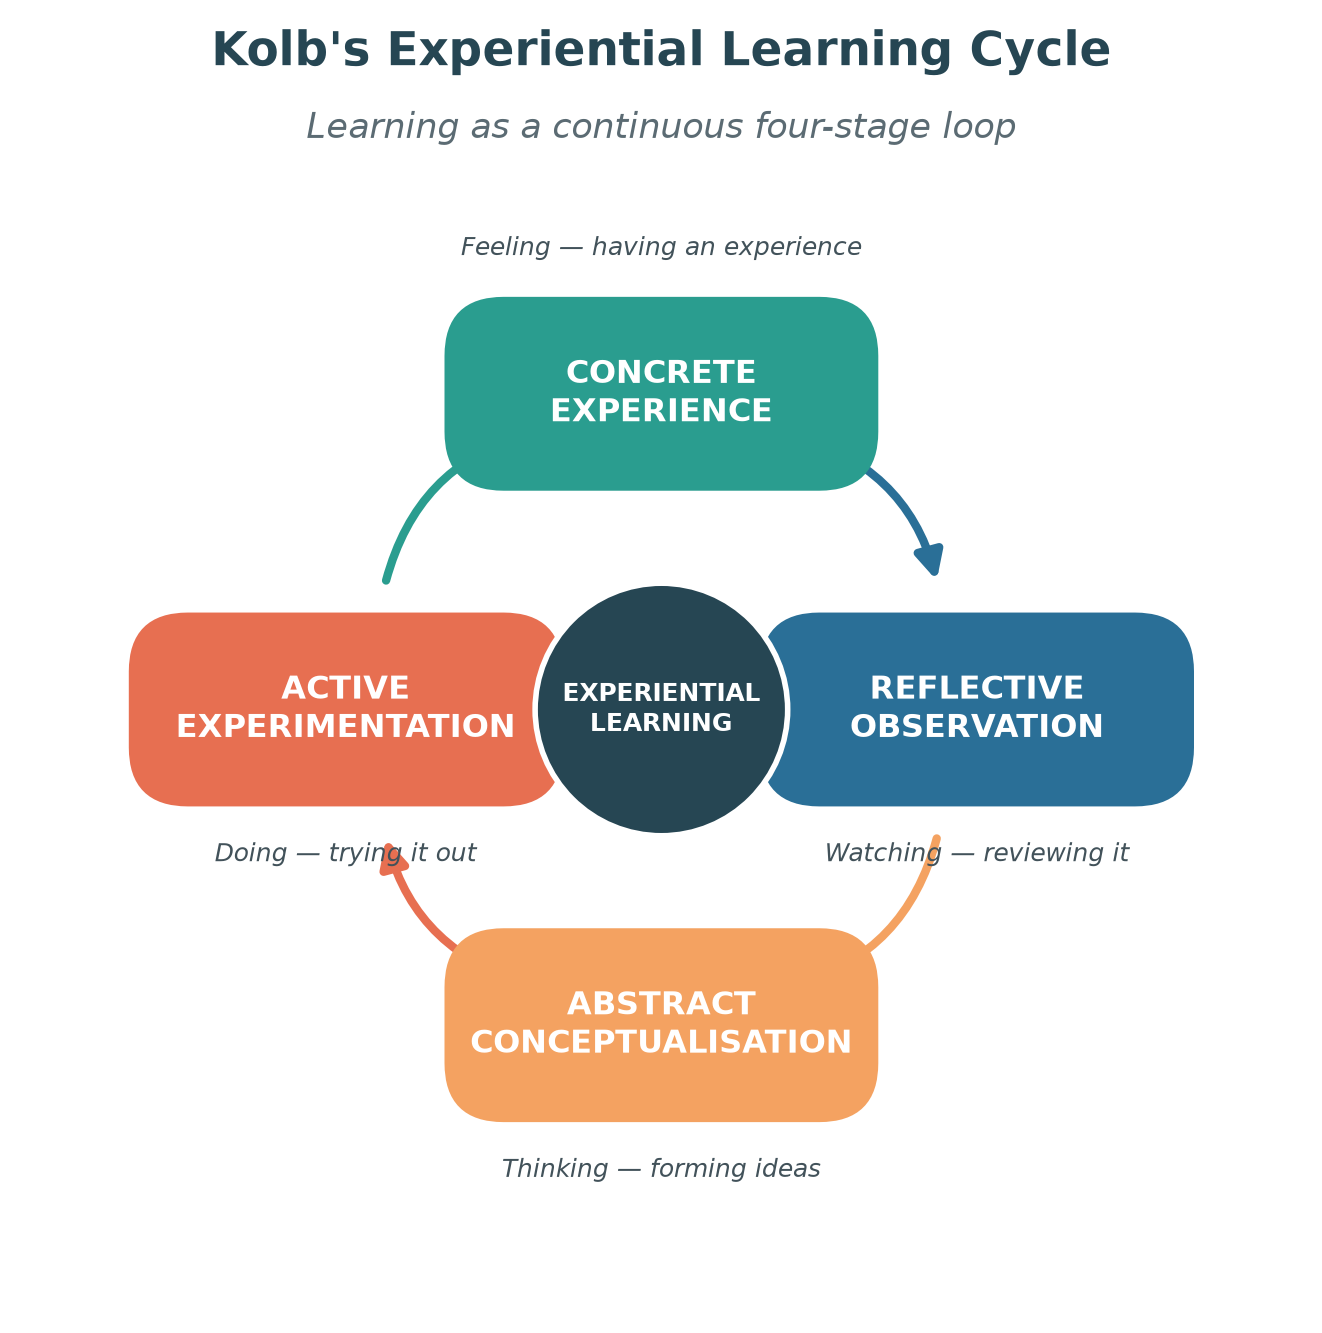
\includegraphics[width=\linewidth]{figures/kolb_cycle.png}
    \end{column}
    \begin{column}{0.45\textwidth}\footnotesize
      Learning is a \kw{continuous cycle} of four stages:
      \begin{enumerate}\footnotesize
        \item \kwt{Concrete Experience} — do / feel.
        \item \kwt{Reflective Observation} — review.
        \item \kwt{Abstract Conceptualisation} — conclude.
        \item \kwt{Active Experimentation} — plan \& try.
      \end{enumerate}
      Effective learning happens when we travel \emph{all the way round} the
      loop — repeatedly.
    \end{column}
  \end{columns}
\end{frame}

\begin{frame}{Kolb's Four Learning Styles}
  \begin{columns}[c]
    \begin{column}{0.58\textwidth}
      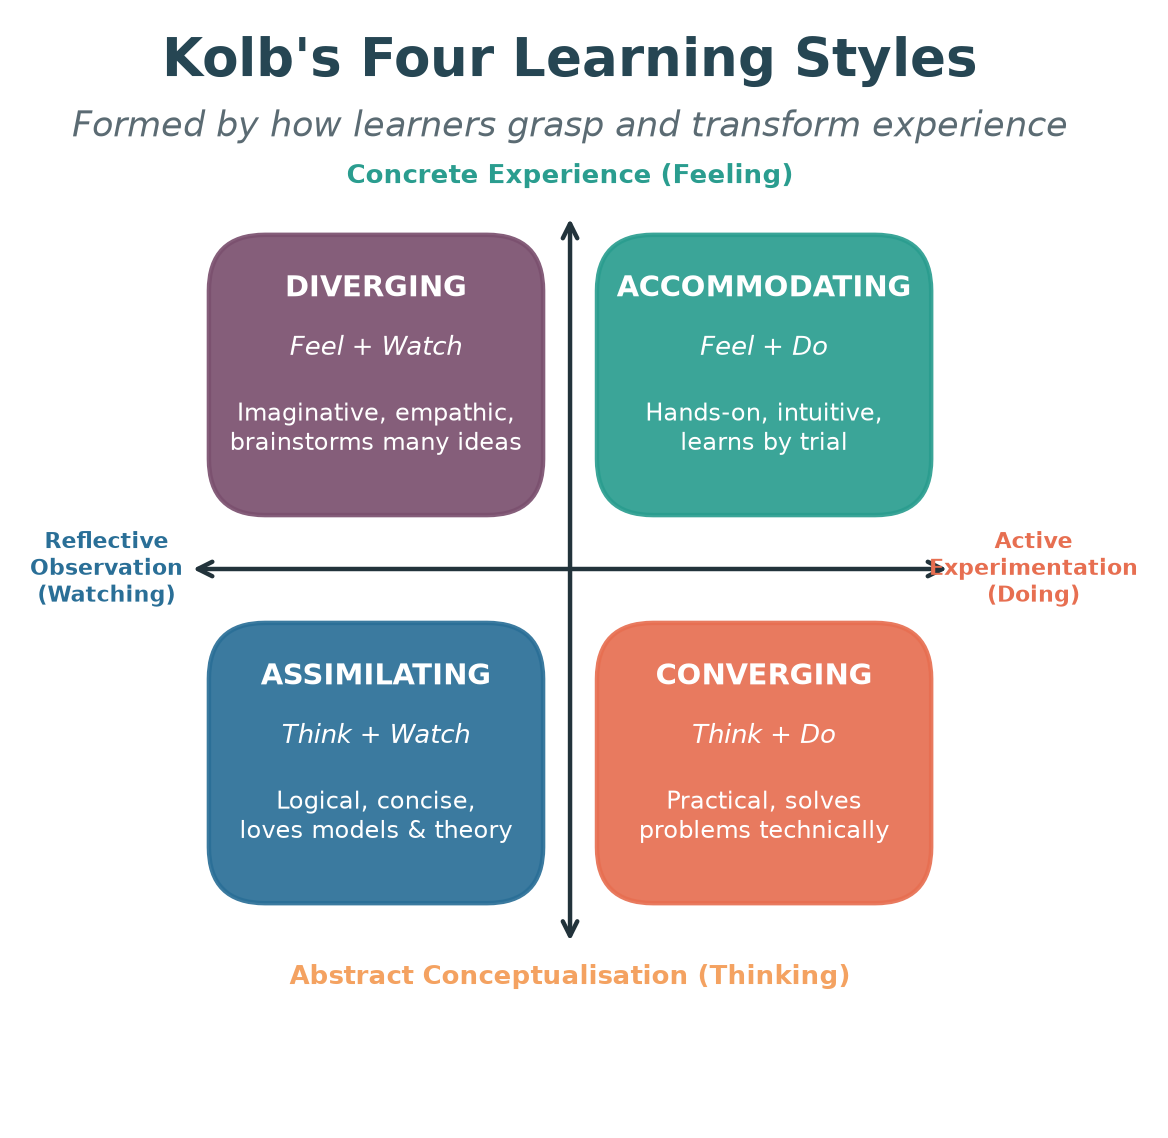
\includegraphics[width=\linewidth]{figures/kolb_styles.png}
    \end{column}
    \begin{column}{0.42\textwidth}\scriptsize
      Combining \emph{how we grasp} and \emph{how we transform} experience
      gives four styles:
      \begin{itemize}\scriptsize
        \item \pill{dtplum}{Diverging} — imaginative, many ideas.
        \item \pill{dtteal}{Accommodating} — hands-on, intuitive.
        \item \pill{dtblue}{Assimilating} — logical, loves theory.
        \item \pill{dtcoral}{Converging} — practical problem-solver.
      \end{itemize}
      \vspace{0.3em}
      Teams work best when \emph{all four styles} are present.
    \end{column}
  \end{columns}
\end{frame}

\begin{frame}{Assessing \& Interpreting Learning Styles}
  \accentrule\\[0.3em]
  \begin{columns}[T]
    \begin{column}{0.5\textwidth}\small
      \textbf{How we assess}
      \begin{itemize}\small
        \item \kw{Learning Style Inventory (LSI)} questionnaires.
        \item Self-reflection journals.
        \item Observation of behaviour in tasks.
      \end{itemize}
    \end{column}
    \begin{column}{0.5\textwidth}\small
      \textbf{How we interpret}
      \begin{itemize}\small
        \item No style is \emph{better} — each has strengths.
        \item Match \kwt{teaching methods} to styles.
        \item Encourage learners to stretch into weaker modes.
      \end{itemize}
    \end{column}
  \end{columns}
  \vspace{0.4em}
  \begin{block}{Application with peers}
    \scriptsize In group projects, deliberately mix styles so ideation,
    analysis, building and testing are all covered.
  \end{block}
\end{frame}

\begin{frame}{The Memory Process}
  \bigfig{memory_process.png}{The information-processing model: sensory $\to$ short-term $\to$ long-term memory.}
\end{frame}

\begin{frame}{Problems in Retention}
  \accentrule\\[0.3em]
  \begin{columns}[T]
    \begin{column}{0.5\textwidth}\small
      Why do we forget?
      \begin{itemize}\small
        \item \kwc{Decay} — traces fade without use.
        \item \kwc{Interference} — old \& new memories clash.
        \item \kwc{Retrieval failure} — no cue to recall.
        \item \kwc{Weak encoding} — shallow processing.
      \end{itemize}
    \end{column}
    \begin{column}{0.5\textwidth}
      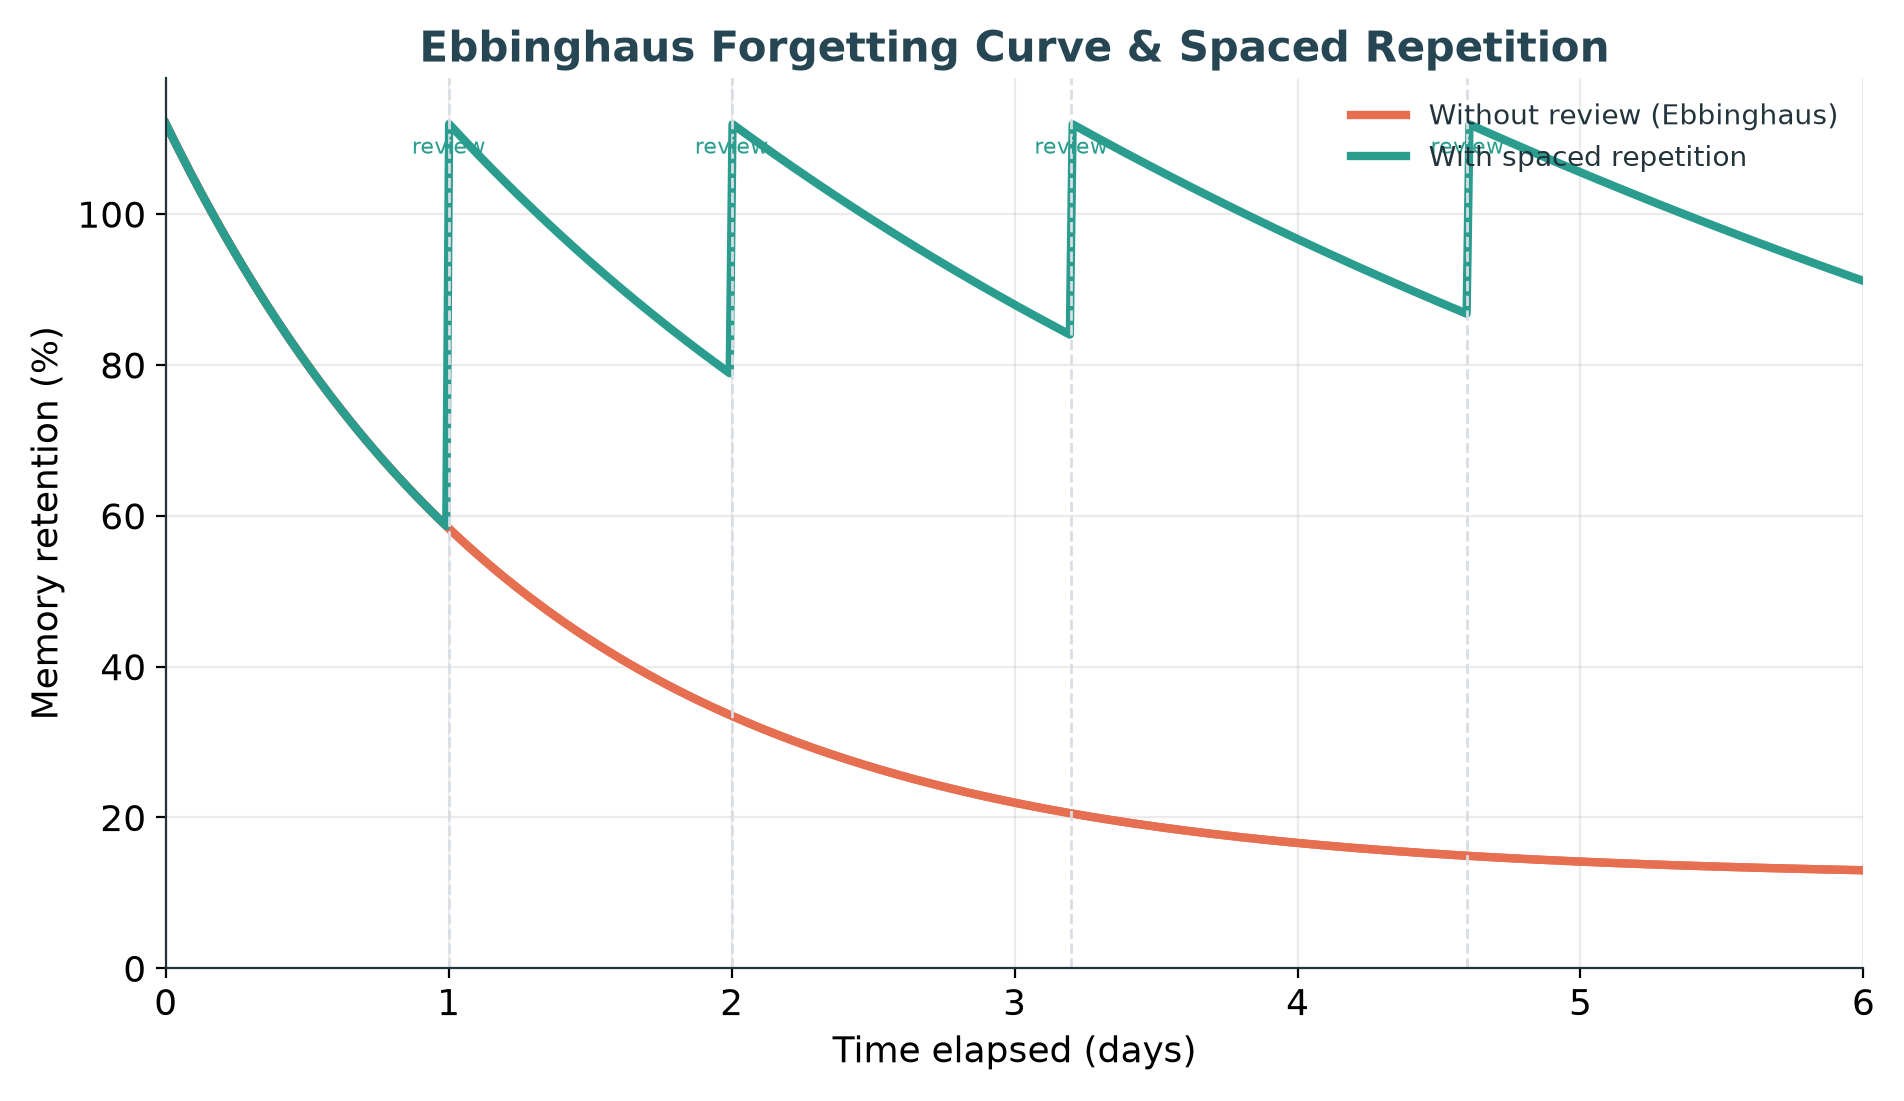
\includegraphics[width=\linewidth]{figures/forgetting_curve.png}
    \end{column}
  \end{columns}
  \vspace{0.2em}
  {\scriptsize The \kw{Ebbinghaus curve} shows rapid forgetting — but each
  review flattens the curve.}
\end{frame}

\begin{frame}{Memory Enhancement Techniques}
  \accentrule\\[0.4em]
  \begin{columns}[T]
    \begin{column}{0.5\textwidth}\small
      \begin{itemize}\small
        \item \kwt{Chunking} — group items into meaningful units.
        \item \kwt{Mnemonics} — acronyms, rhymes, imagery.
        \item \kwt{Spaced repetition} — review at intervals.
        \item \kwt{Elaboration} — connect to prior knowledge.
      \end{itemize}
    \end{column}
    \begin{column}{0.5\textwidth}\small
      \begin{itemize}\small
        \item \kwt{Dual coding} — words + visuals together.
        \item \kwt{Active recall} — test yourself, don't re-read.
        \item \kwt{Method of loci} — memory "palace".
        \item \kwt{Sleep \& rest} — consolidate memories.
      \end{itemize}
    \end{column}
  \end{columns}
  \vspace{0.4em}
  \begin{block}{Design tip}\scriptsize
    Good product design \emph{reduces the memory load} on the user — clear
    labels, consistent layouts and helpful cues.
  \end{block}
\end{frame}

\begin{frame}{Emotions, Experience \& Expression}
  \accentrule\\[0.3em]
  \begin{columns}[T]
    \begin{column}{0.55\textwidth}\small
      Emotions shape how people \kw{experience} and \kw{remember} products.
      \begin{itemize}\small
        \item \kwt{Emotion} — an internal feeling (joy, frustration, trust).
        \item \kwt{Experience} — the felt journey of using something.
        \item \kwt{Expression} — how emotion is shown \& communicated.
      \end{itemize}
      \vspace{0.3em}
      Peak emotions (delight or annoyance) leave the strongest memories —
      the \emph{peak-end rule}.
    \end{column}
    \begin{column}{0.45\textwidth}
      \begin{block}{Emotional design (Norman)}\scriptsize
        \begin{itemize}\scriptsize
          \item \textbf{Visceral} — first look \& feel.
          \item \textbf{Behavioural} — pleasure of use.
          \item \textbf{Reflective} — meaning \& self-image.
        \end{itemize}
      \end{block}
    \end{column}
  \end{columns}
\end{frame}

\begin{frame}{Empathy \& Emotional Intelligence}
  \begin{columns}[c]
    \begin{column}{0.6\textwidth}
      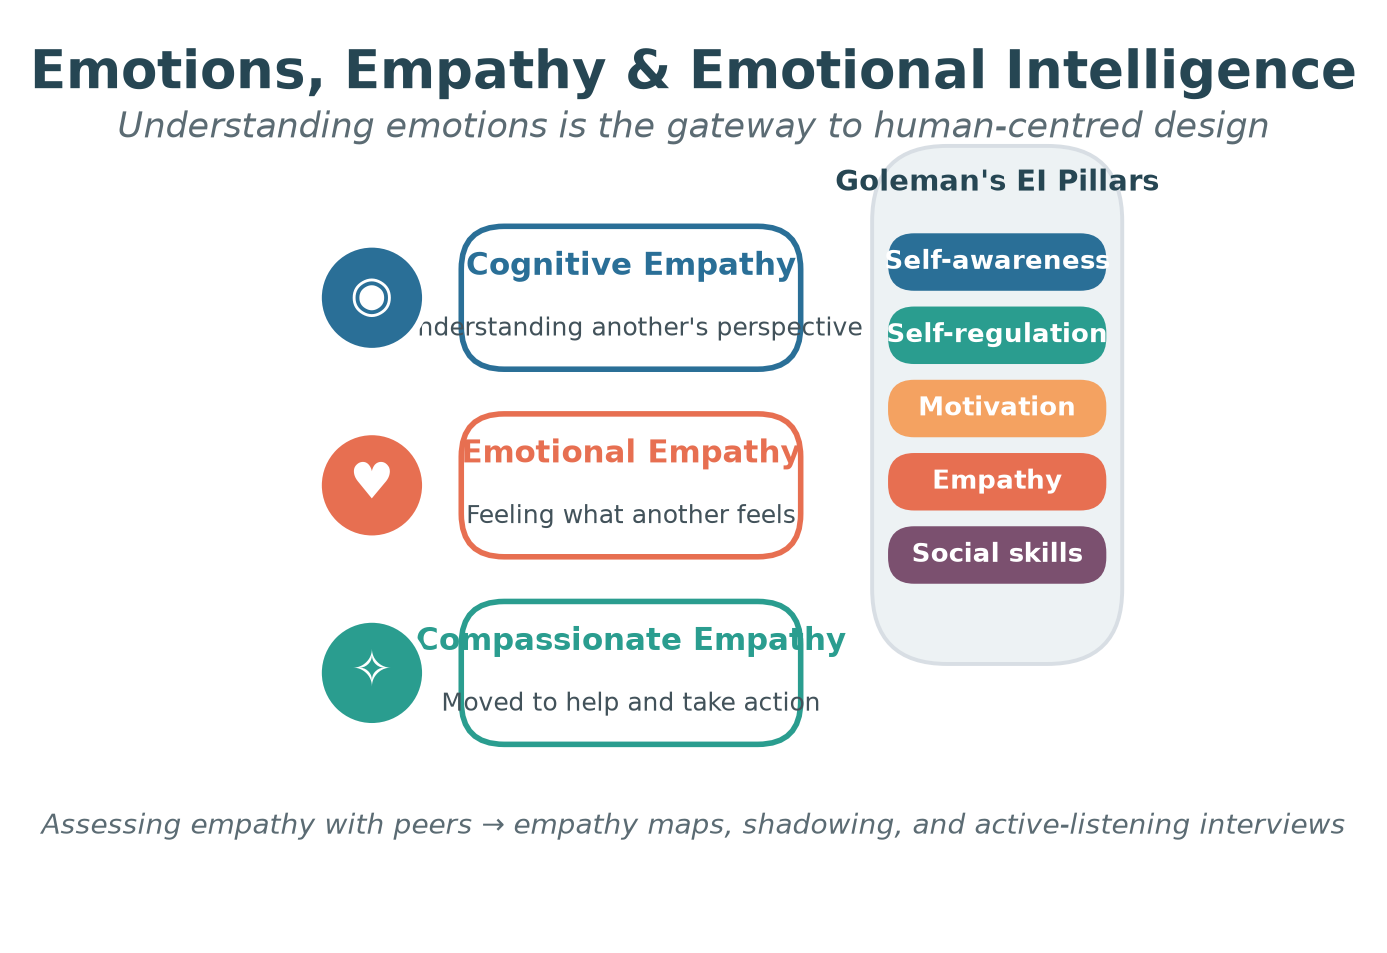
\includegraphics[width=\linewidth]{figures/empathy.png}
    \end{column}
    \begin{column}{0.4\textwidth}\scriptsize
      \kw{Empathy} — the ability to understand and share another's feelings —
      is the \emph{heart of design thinking}.
      \vspace{0.3em}
      \textbf{Assessing empathy with peers}
      \begin{itemize}\scriptsize
        \item Empathy maps (says / thinks / does / feels).
        \item Shadowing \& observation.
        \item Active-listening interviews.
      \end{itemize}
    \end{column}
  \end{columns}
\end{frame}

%% Requires the macros/colours defined in main.tex's preamble.

%==============================================================================
\section{An Insight to Learning}
%==============================================================================
\unitdivider{I}{An Insight to Learning}{Learning, memory, emotion \& empathy}

\begin{frame}{Understanding the Learning Process}
  \accentrule\\[0.3em]
  \begin{columns}[T]
    \begin{column}{0.58\textwidth}\small
      Learning is the process of acquiring \kw{knowledge}, \kw{skills} and
      \kw{attitudes} through experience, study or teaching.
      \begin{itemize}\small
        \item \kwt{Cognitive} — thinking, understanding, problem solving.
        \item \kwt{Affective} — emotions, values, motivation.
        \item \kwt{Psychomotor} — physical / hands-on skills.
      \end{itemize}
      \vspace{0.3em}
      Effective designers are \emph{lifelong learners}: they observe, reflect,
      conceptualise and experiment — exactly the loop Kolb described.
    \end{column}
    \begin{column}{0.42\textwidth}
      \begin{block}{Why it matters for design}
        \scriptsize
        Understanding \emph{how humans learn} helps us design products,
        instructions and experiences that people can pick up quickly and use
        intuitively.
      \end{block}
    \end{column}
  \end{columns}
\end{frame}

\begin{frame}{Kolb's Experiential Learning Cycle}
  \begin{columns}[c]
    \begin{column}{0.55\textwidth}
      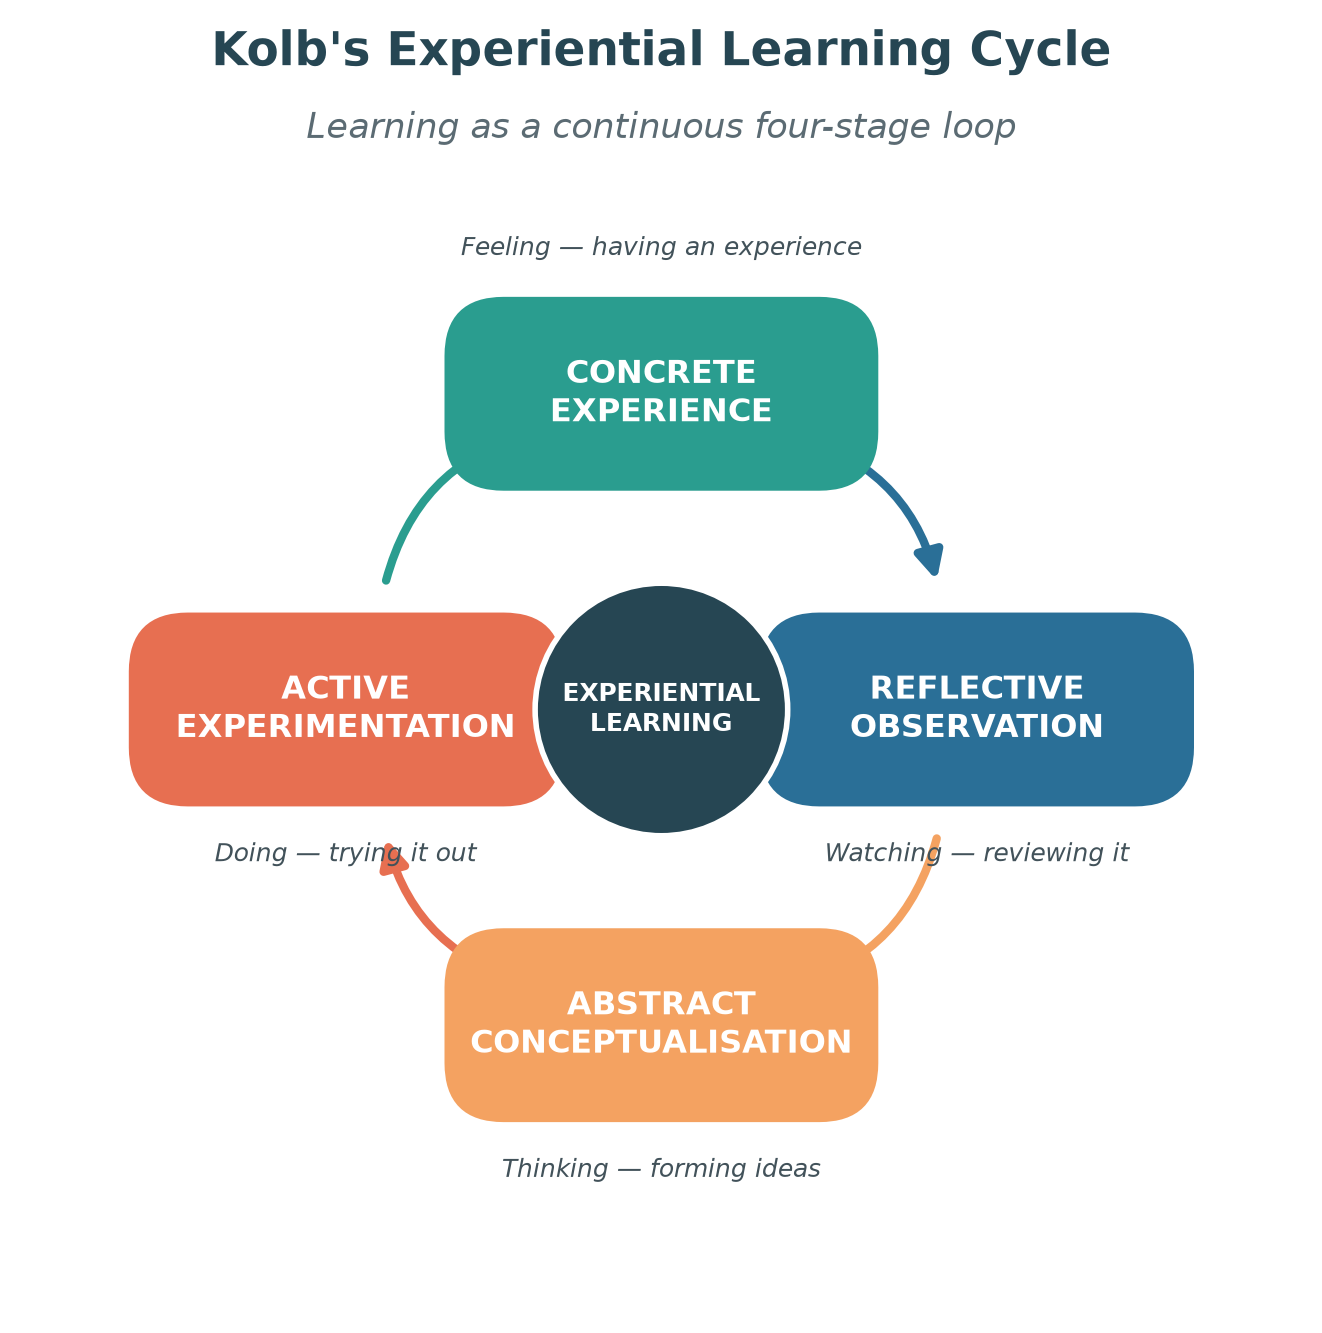
\includegraphics[width=\linewidth]{figures/kolb_cycle.png}
    \end{column}
    \begin{column}{0.45\textwidth}\footnotesize
      Learning is a \kw{continuous cycle} of four stages:
      \begin{enumerate}\footnotesize
        \item \kwt{Concrete Experience} — do / feel.
        \item \kwt{Reflective Observation} — review.
        \item \kwt{Abstract Conceptualisation} — conclude.
        \item \kwt{Active Experimentation} — plan \& try.
      \end{enumerate}
      Effective learning happens when we travel \emph{all the way round} the
      loop — repeatedly.
    \end{column}
  \end{columns}
\end{frame}

\begin{frame}{Kolb's Four Learning Styles}
  \begin{columns}[c]
    \begin{column}{0.58\textwidth}
      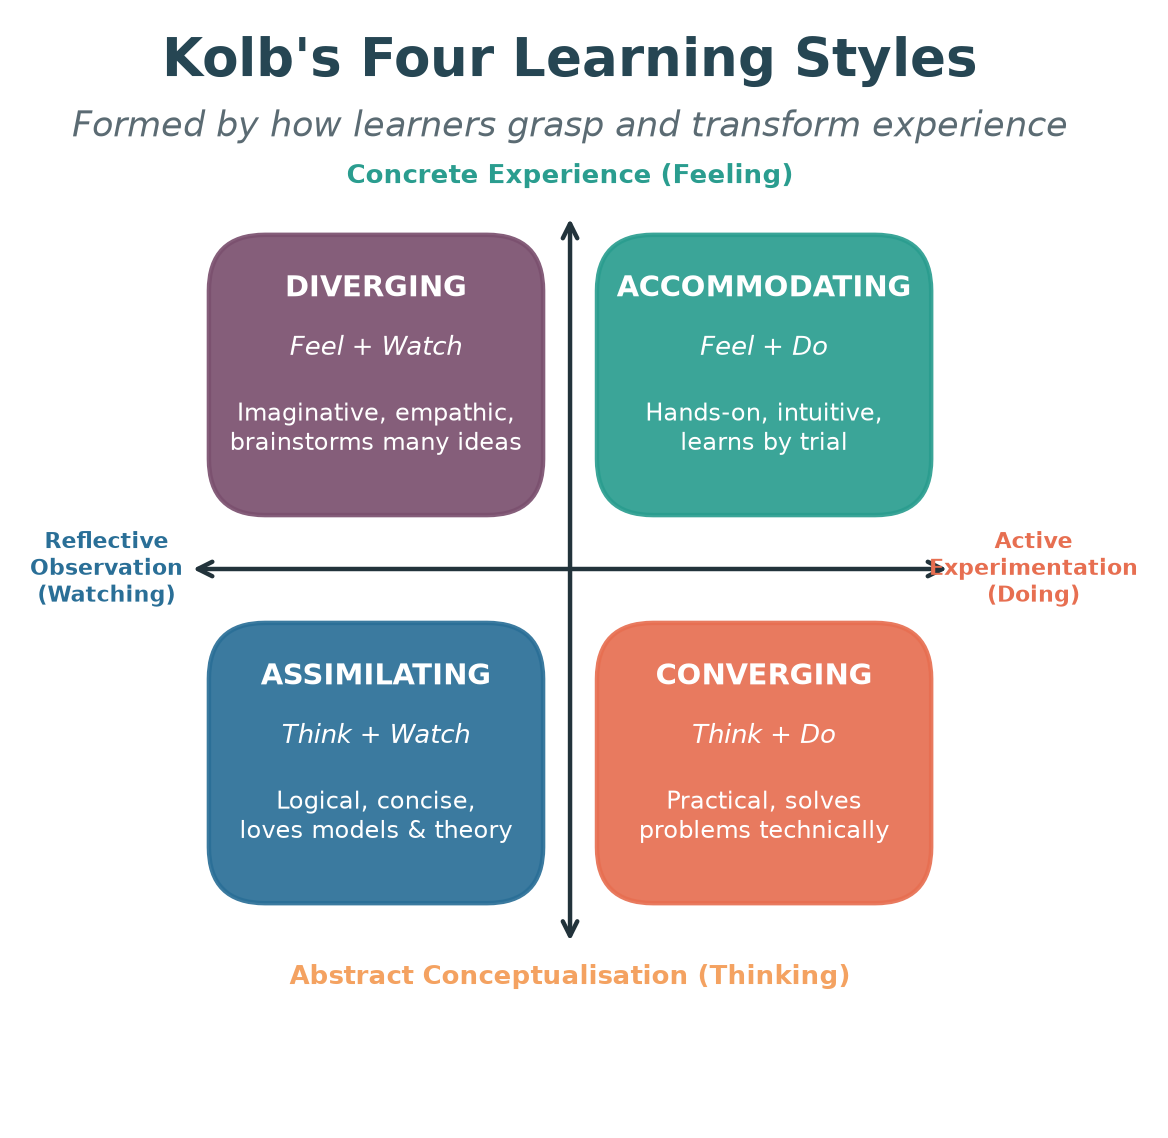
\includegraphics[width=\linewidth]{figures/kolb_styles.png}
    \end{column}
    \begin{column}{0.42\textwidth}\scriptsize
      Combining \emph{how we grasp} and \emph{how we transform} experience
      gives four styles:
      \begin{itemize}\scriptsize
        \item \pill{dtplum}{Diverging} — imaginative, many ideas.
        \item \pill{dtteal}{Accommodating} — hands-on, intuitive.
        \item \pill{dtblue}{Assimilating} — logical, loves theory.
        \item \pill{dtcoral}{Converging} — practical problem-solver.
      \end{itemize}
      \vspace{0.3em}
      Teams work best when \emph{all four styles} are present.
    \end{column}
  \end{columns}
\end{frame}

\begin{frame}{Assessing \& Interpreting Learning Styles}
  \accentrule\\[0.3em]
  \begin{columns}[T]
    \begin{column}{0.5\textwidth}\small
      \textbf{How we assess}
      \begin{itemize}\small
        \item \kw{Learning Style Inventory (LSI)} questionnaires.
        \item Self-reflection journals.
        \item Observation of behaviour in tasks.
      \end{itemize}
    \end{column}
    \begin{column}{0.5\textwidth}\small
      \textbf{How we interpret}
      \begin{itemize}\small
        \item No style is \emph{better} — each has strengths.
        \item Match \kwt{teaching methods} to styles.
        \item Encourage learners to stretch into weaker modes.
      \end{itemize}
    \end{column}
  \end{columns}
  \vspace{0.4em}
  \begin{block}{Application with peers}
    \scriptsize In group projects, deliberately mix styles so ideation,
    analysis, building and testing are all covered.
  \end{block}
\end{frame}

\begin{frame}{The Memory Process}
  \bigfig{memory_process.png}{The information-processing model: sensory $\to$ short-term $\to$ long-term memory.}
\end{frame}

\begin{frame}{Problems in Retention}
  \accentrule\\[0.3em]
  \begin{columns}[T]
    \begin{column}{0.5\textwidth}\small
      Why do we forget?
      \begin{itemize}\small
        \item \kwc{Decay} — traces fade without use.
        \item \kwc{Interference} — old \& new memories clash.
        \item \kwc{Retrieval failure} — no cue to recall.
        \item \kwc{Weak encoding} — shallow processing.
      \end{itemize}
    \end{column}
    \begin{column}{0.5\textwidth}
      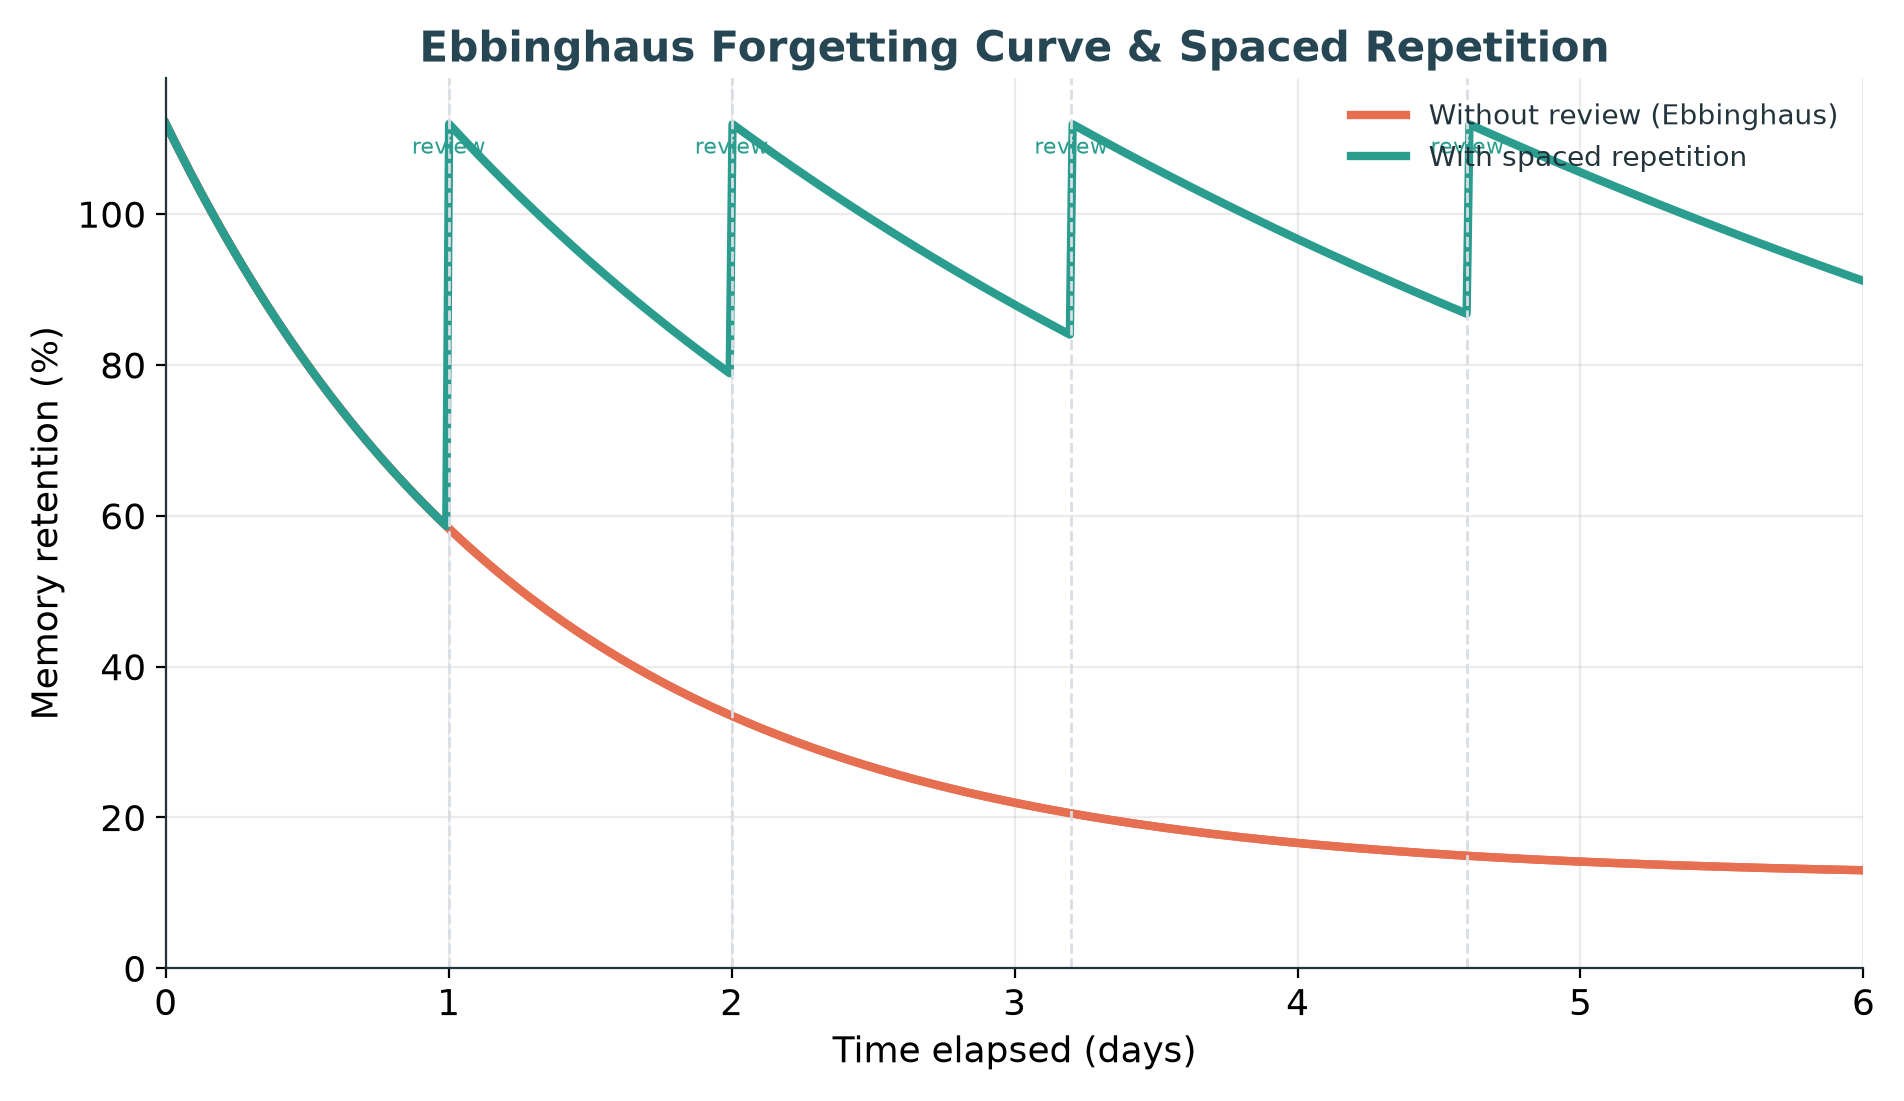
\includegraphics[width=\linewidth]{figures/forgetting_curve.png}
    \end{column}
  \end{columns}
  \vspace{0.2em}
  {\scriptsize The \kw{Ebbinghaus curve} shows rapid forgetting — but each
  review flattens the curve.}
\end{frame}

\begin{frame}{Memory Enhancement Techniques}
  \accentrule\\[0.4em]
  \begin{columns}[T]
    \begin{column}{0.5\textwidth}\small
      \begin{itemize}\small
        \item \kwt{Chunking} — group items into meaningful units.
        \item \kwt{Mnemonics} — acronyms, rhymes, imagery.
        \item \kwt{Spaced repetition} — review at intervals.
        \item \kwt{Elaboration} — connect to prior knowledge.
      \end{itemize}
    \end{column}
    \begin{column}{0.5\textwidth}\small
      \begin{itemize}\small
        \item \kwt{Dual coding} — words + visuals together.
        \item \kwt{Active recall} — test yourself, don't re-read.
        \item \kwt{Method of loci} — memory "palace".
        \item \kwt{Sleep \& rest} — consolidate memories.
      \end{itemize}
    \end{column}
  \end{columns}
  \vspace{0.4em}
  \begin{block}{Design tip}\scriptsize
    Good product design \emph{reduces the memory load} on the user — clear
    labels, consistent layouts and helpful cues.
  \end{block}
\end{frame}

\begin{frame}{Emotions, Experience \& Expression}
  \accentrule\\[0.3em]
  \begin{columns}[T]
    \begin{column}{0.55\textwidth}\small
      Emotions shape how people \kw{experience} and \kw{remember} products.
      \begin{itemize}\small
        \item \kwt{Emotion} — an internal feeling (joy, frustration, trust).
        \item \kwt{Experience} — the felt journey of using something.
        \item \kwt{Expression} — how emotion is shown \& communicated.
      \end{itemize}
      \vspace{0.3em}
      Peak emotions (delight or annoyance) leave the strongest memories —
      the \emph{peak-end rule}.
    \end{column}
    \begin{column}{0.45\textwidth}
      \begin{block}{Emotional design (Norman)}\scriptsize
        \begin{itemize}\scriptsize
          \item \textbf{Visceral} — first look \& feel.
          \item \textbf{Behavioural} — pleasure of use.
          \item \textbf{Reflective} — meaning \& self-image.
        \end{itemize}
      \end{block}
    \end{column}
  \end{columns}
\end{frame}

\begin{frame}{Empathy \& Emotional Intelligence}
  \begin{columns}[c]
    \begin{column}{0.6\textwidth}
      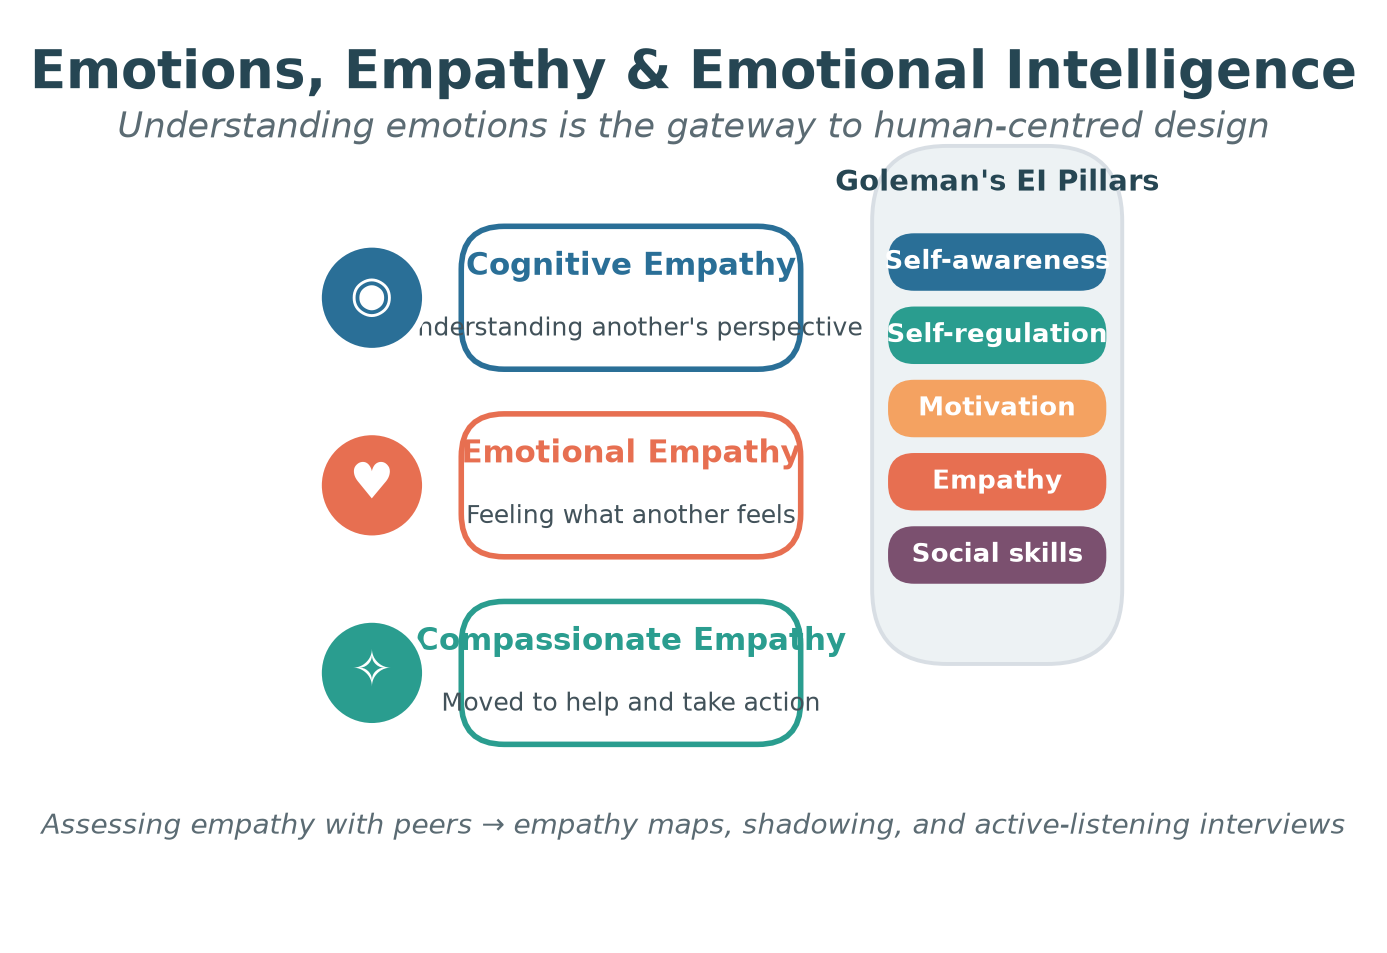
\includegraphics[width=\linewidth]{figures/empathy.png}
    \end{column}
    \begin{column}{0.4\textwidth}\scriptsize
      \kw{Empathy} — the ability to understand and share another's feelings —
      is the \emph{heart of design thinking}.
      \vspace{0.3em}
      \textbf{Assessing empathy with peers}
      \begin{itemize}\scriptsize
        \item Empathy maps (says / thinks / does / feels).
        \item Shadowing \& observation.
        \item Active-listening interviews.
      \end{itemize}
    \end{column}
  \end{columns}
\end{frame}
